\documentclass[a4paper, twoside]{article}
\usepackage[utf8]{inputenc} % Especifica la codificación de caracteres de los documentos.
\usepackage[spanish]{babel} % Indica que el documento se escribirá en español.
\usepackage[top=3cm, bottom=2.5cm, inner=1.5cm, outer=2.5cm]{geometry} % Márgenes personalizados
\usepackage{subfiles} % Paquete para incluir el preambulo en los sub archivos.
\usepackage{afterpage} % Permite añadir páginas despues de una página dada.
\usepackage{hyperref} % Permite incluir enlaces en los archivos.
\usepackage{lastpage} % Paquete para poder contabilizar el total de páginas del documento.
\usepackage{fancyhdr} % Permite personalizar los header y footer del documento.
\usepackage{amsmath} % Comandos para la escritura de fórmulas matemáticas de mayor complejidad
\usepackage{amsfonts} % Proporciona fuentes matemáticas
\usepackage{amssymb} % Proporciona símbolos matemáticos de la American Mathematical Society
\usepackage{graphicx} % Permite incluir gráficos
\usepackage[hang, bf]{caption} % Personaliza los subtítulos de las figuras y tablas
\usepackage{float} % Permite posicionar mejor las figuras y tablas
\usepackage{pgf,tikz}
\usepackage{environ}

% Defino la ruta de los paquetes personalizados para el apunte
\newcommand{\rutapaquetes}{./paquetes-apunte}

\usepackage[mostrarlicencia]{\rutapaquetes/caratula} % Caratula personalizada (cargada desde caratula.sty)
\usepackage[ocultarrevisores]{\rutapaquetes/colaboradores} % Seccion de colaboradores (cargada y creada con colaboradores.sty)
\usepackage{\rutapaquetes/historial} % Seccion de historial de cambios (cargada y creada con historial.sty)

% Define los estilos de los enlaces interpretados por el paquete hyperref
\hypersetup{
	colorlinks=true,% false: boxed links; true: colored links
	linkcolor=black,% color of internal links (change box color with linkbordercolor)
	citecolor=green,% color of links to bibliography
	filecolor=magenta, % color of file links
	urlcolor=blue,	 % color of external links
}

\newcommand{\imgdir}{../resources/images} % Ruta de las imágenes

% Define los directorios de las imágenes y gráficos
\graphicspath{ {\imgdir/} {\rutapaquetes/} }

\newcommand{\nombremateria}{Álgebra II (61.08 - 81.02)} % Defino el comando "\nombremateria" para no harcodear el nombre en varios lugares.

% Define el pagestyle personalizado
\pagestyle{fancy}
\fancyhf{}
\renewcommand{\sectionmark}[1]{\markboth{}{\thesection\ \ #1}}
% Define header para pagina par
\fancyhead[ER]{\rightmark}
% Define header para pagina impar
\fancyhead[OL]{\rightmark}
% Define footer para pagina par
\fancyfoot[EL]{\nombremateria \hspace{0.1cm} - Resumen} % Nombre del apunte a la izquierda
\fancyfoot[ER]{Página \thepage\ de \pageref{LastPage}} % Numero de pagina a la derecha
% Define footer para pagina impar
\fancyfoot[OL]{Página \thepage\ de \pageref{LastPage}} % Numero de pagina a la izquierda
\fancyfoot[OR]{\nombremateria \hspace{0.1cm} - Resumen} % Nombre del apunte a la derecha

\renewcommand{\footrulewidth}{0.4pt} % Agrego linea que separa el footer

% Configura la caratula
\materia{\nombremateria}
\tipoapunte{Resumen}
%\tema{Tema de la Materia}
%\subtema{Subtema}

\numberwithin{equation}{section}
\numberwithin{figure}{section}
\numberwithin{table}{section}

\pdfcompresslevel=9

\everymath{\displaystyle}
\newcommand{\vect}[1]{\overline{\textbf{#1}}}
\newcommand{\bayes}{\mathop{\lessgtr}}

\newcommand{\fil}[1]{\text{Fil}(#1)}
\newcommand{\col}[1]{\text{Col}(#1)}
\newcommand{\nul}[1]{\text{Nul}(#1)}
\newcommand{\im}[1]{\text{Im}(#1)}
\newcommand{\rg}[1]{\text{rango}\left(#1\right)}
\newcommand{\dime}[1]{\text{Dim}(#1)}
\newcommand{\dete}[1]{\left\vert #1 \right\vert}
\newcommand{\tr}[1]{\text{tr}(#1)}
\newcommand{\gen}[1]{\text{gen}\left\{#1\right\}}
\newcommand{\produ}[1]{(#1)}

\usetikzlibrary{shapes, arrows, positioning, shadows, trees, automata}

\tikzstyle{definicion} = [draw=red, fill=gray!20, very thick,rectangle, rounded corners, inner sep=10pt, inner ysep=20pt]
\tikzstyle{fancytitle} =[fill=red, text=white]

\tikzstyle{corolario} = [draw=red, fill=green!20, very thick,rectangle, rounded corners, inner sep=10pt, inner ysep=20pt]
\tikzstyle{fancytitle} =[fill=red, text=white]

\tikzstyle{teorema} = [draw=red, fill=blue!20, very thick,rectangle, rounded corners, inner sep=10pt, inner ysep=20pt]
\tikzstyle{fancytitle} =[fill=red, text=white]

\NewEnviron{corolario}[1]{%
  \begin{tikzpicture}
    \node [corolario] (box){%
      \begin{minipage}{0.80\textwidth}
       \BODY
        \end{minipage}};
    \node[fancytitle, right=10pt] at (box.north west) {#1};
    \node[fancytitle, rounded corners] at (box.south) {$\aleph$};
   \end{tikzpicture}
}

\NewEnviron{definicion}[1]{%
  \begin{tikzpicture}
    \node [definicion] (box){%
      \begin{minipage}{0.80\textwidth}
       \BODY
        \end{minipage}};
    \node[fancytitle, right=10pt] at (box.north west) {#1};
    \node[fancytitle, rounded corners] at (box.south) {$\aleph$};
   \end{tikzpicture}
}
%------------------------- Inicio del documento ---------------------------

\begin{document}

\maketitle % Carátula

\tableofcontents % Índice de contenido
%\listoffigures % Índice de figuras
%\listoftables % Índice de tablas

\subfile{\rutapaquetes/sobre-el-proyecto.tex} % Inlcuye informacion sobre el proyecto FIUBA Apuntes

\section{Matrices}
\subsection{Propiedades generales}
\begin{corolario}{Propiedades de matrices}
  Dadas las matrices $A,B,C$ se tiene que:\\
  
    \begin{minipage}{0.4\textwidth}
    \begin{itemize}
      \item $A+B=B+A$
      \item $A+(B+C)=(A+B)+C$
      \item $\alpha(A+B)=\alpha A+\alpha B$
      \item $(\alpha+\beta)A=\alpha A+\beta A$
      \item $\alpha\left(\beta A\right)=(\alpha\beta)A$
      \item $A+0_n=A$
    \end{itemize}
    \end{minipage}
    \begin{minipage}{0.4\textwidth}
      \begin{itemize}
        \item $A+(-A)=0_n$
        \item $A(B+C)=AB+AC$
        \item $(A+B)C=AC+BC$
        \item $A(BC)=(AB)C$
        \item $\alpha(AB)=(\alpha A)B=A(\alpha B)$
        \item $A 0_n=0_n$
      \end{itemize}
    \end{minipage}
 
\end{corolario}



\subsection{Propiedades de la inversa, la traza y la traspuesta}
\begin{corolario}{Propiedades de matrices}
  Dadas las matrices $A,B,C$ se tiene que:\\
  
  \begin{minipage}{0.3\textwidth}
    Propiedades de la inversa:
    \begin{itemize}
      \item $\left(A^{-1}\right)^{-1}$
      \item $\left(AB\right)^{-1}=B^{-1}A^{-1}$
      \item $\left(\alpha A\right)^{-1}=\frac{A^{-1}}{\alpha}, \alpha \neq 0$
      \item $\left(A^n\right)^{-1}=\left(A^{-1}\right)^n$
      \item $A^{-1}=\frac{\text{adj}(A)}{\dete{A}}$
    \end{itemize}
    \end{minipage}
    \begin{minipage}{0.3\textwidth}
    Propiedades de la traza:
    \begin{itemize}
      \item $\tr{A+B}=\tr{A}+\tr{B}$
      \item $\tr{AB}=\tr{BA}$
      \item $\tr{\alpha A}=\alpha \tr{A}$
      \item $\tr{A^T}=\tr{A}$
    \end{itemize}
    \end{minipage}
    \begin{minipage}{0.3\textwidth}
    Propiedades de la traspuesta:
      \begin{itemize}
        \item $\left(A+B\right)^T=A^T+B^T$
        \item $\left(AB\right)^T=B^T A^T$
        \item $\left(A^T\right)^T=A$
        \item $\left(\alpha A\right)^T=\alpha A^T$
        \item $\left(A^T\right)^{-1}=\left(A^{-1}\right)^T$
      \end{itemize}
    \end{minipage}
\end{corolario}

\subsection{Propiedades de los determinantes}
\begin{corolario}{Propiedades de determinantes}
  Sean $A,B \in R^{n \times m}$
  \begin{align}
    \dete{A^T}=\dete{A} \\
	\dete{AB}=\dete{A} \dete{B}
  \end{align}
  Si $B$ la obtengo de sumar k veces una fila de $A$ sobre otra:
  \begin{align}
    \dete{B}=\dete{A}
  \end{align}
  Si $B$ la obtengo de intercambiar $k$ veces las fila de $A$:
  \begin{align}
    \dete{B}=(-1)^k\dete{A}
  \end{align}
  Si $B$ la obtengo de multiplicar por $k$, $n$ veces las filas de A:
  \begin{align}
    \dete{B}=k^n\dete{A}
  \end{align}
  Si $A$ es una matriz triangular:
  \begin{align}
    \dete{A}=\prod_{i=1}^n a{ii}
  \end{align}
\end{corolario}

\subsection{Subespacios fila, columna y null}
\begin{definicion}{Espacio fila,columna y nulo de matrices}
  Sean $A \in R^{n \times m} \text{ , } B \in R^{r \times n}$, se define:
  \begin{itemize}
	\item	\textbf{Espacio Fila:} $\text{Fif}(A)=\{x \in R^m \vert x \text{ es combinación lineal de las filas de } A\}$
	\item \textbf{Espacio Columna:} $\text{Col}(A)=\{b \in R^n \vert Ax=b \text{ para alguna x}\}$
	\item \textbf{Espacio nulo:} $\text{Nul}(A)=\{x \in R^m \vert Ax=0\}$
  \end{itemize}
\end{definicion}

\begin{corolario}{Propiedades de los espacios definidos}
  Propiedades:
  \begin{align}
	\nul{A}=\nul{A^T A}=\fil{A}^\bot \\
	\nul{A^T}=\nul{A A^T}=\col{A}^\bot \\
	\rg{A}=\rg{A^T A} \Rightarrow A^T A \\
	\dime{\col{A}}=\dime{\fil{A}} \\
	\col{A} \bigotimes \col{A}^\bot=R^n \\
	\fil{A} \bigotimes \fil{A}^\bot=R^m \\
	\rg{A}+\dim{\nul{A}}=m \\	
	\col{BA} \subseteq \col{B} \text{, Iguales si } \rg{A}=n \\
	\nul{A} \subseteq \nul{BA} \text{, Iguales si } \rg{B}=n \\
	\text{Si } \rg{A}=n \Rightarrow \rg{BA}=\rg{B} \\
	\text{Si } \rg{B}=n \Rightarrow \rg{BA}=\rg{A} \\
    \col{A} \bot \col{B} \Leftrightarrow A^T B=0
  \end{align}
  De \textbf{(1.15)} se ve que $A^T A \text{ invertible } \longleftrightarrow A \text{ invertible}$
\end{corolario}

\begin{definicion}{Matrices equivalentes}
  Dos matrices $A$ y $B$ son equivalentes si existen otras dos matrices $E$ y $F$ regulares tal que:
    \begin{align}
      A=EBF
	\end{align}
	Dos matrices equivalentes pueden pensarse como dos descripciones de una misma Transformación Lineal, pero con respecto a bases distintas.
\end{definicion}

\begin{definicion}{Matrices Semejantes}
  Dos matrices cuadradas $A$ y $B$ son semejantes (notamos $A \sim B$) si y solo si existe una matriz $P$ inversible tal que:
    \begin{align}
      B=P^{-1}AP \text{ ,ó}\\
      A=PBP^{-1}
    \end{align}
\end{definicion}

\begin{corolario}{Propiedades de matrices semejantes}
  Dos matrices semejantes pueden pensarse como dos descripciones de un mismo operador lineal, pero con respecto a bases distintas. Estas dos matrices cumplen que:
    \begin{align}
      \dete{A}=\dete{B} \\
      \tr{A}=\tr{B} \\
      \rg{A}=\rg{B} \\
      p_A(\lambda)=p_B(\lambda) \Rightarrow \sigma(A)=\sigma(B)
	\end{align}
\end{corolario}

\newpage
\section{Espacios vectoriales}
\subsection{Propiedades de los subespacios}
\begin{tikzpicture}
	\node [corolario] (box){%
		\begin{minipage}{0.80\textwidth}
			$S$ es un subespacio vectorial del espacio $V_K$ si y solo si:
			\begin{align}
				0_V \in S \\
				(\alpha X+Y) \in S, \forall X,Y \in V \text{ y } \forall \alpha \in K
			\end{align}
		\end{minipage}};
	\node[fancytitle, right=10pt] at (box.north west) {Propiedades de los subespacios};
	\node[fancytitle, rounded corners] at (box.south) {$\aleph$};
\end{tikzpicture}

\subsection{Independencia lineal}
\begin{tikzpicture}
	\node [definicion] (box){%
		\begin{minipage}{0.80\textwidth}
			El vector $\vect{x}$ es una combinación lineal de $\vect{v}_1,\vect{v}_2,\ldots,\vect{v}_n$ si:
			\begin{align}
				\vect{x}=\sum_{i=1}^n \alpha_i v_i
			\end{align}
			Y si $a_1,\ldots,a_n$ no son todos nulos.
		\end{minipage}};
	\node[fancytitle, right=10pt] at (box.north west) {Combinación lineal};
	\node[fancytitle, rounded corners] at (box.south) {$\aleph$};
\end{tikzpicture}

\begin{tikzpicture}
	\node [definicion] (box){%
		\begin{minipage}{0.80\textwidth}
			$\vect{x}$ es \textbf{linealmente independiente} si:
			\begin{align}
				\sum_{i=1}^n \alpha_i v_i=0 \text{ , y} \\
				a_i=0 \forall i
			\end{align}
			Dos vectores son \textbf{linealmente dependientes} si son proporcionales. Un subconjunto de un conjunto linealmente dependiente sigue siendo linealmente dependiente
		\end{minipage}};
	\node[fancytitle, right=10pt] at (box.north west) {Independencia lineal};
	\node[fancytitle, rounded corners] at (box.south) {$\aleph$};
\end{tikzpicture}

\subsection{Operaciones con subespacios}
\begin{tikzpicture}
	\node [corolario] (box){%
		\begin{minipage}{0.80\textwidth}
			\begin{itemize}
				\item \textbf{Intersección:} $S=\bigcap_{i=1}^n S_i=\{ \vect{x} \in V \vert \vect{x} \in S_i \text{ , } \forall i=1,\ldots,n \}$
				\item \textbf{Suma:} $S=\sum_{i=1}^n S_i=\gen{\bigcup_{i=1}^m B_i}$, donde $B_i$ es una base de $S_i$
				\item \textbf{Unión:} $S=S_1 \cup S_2$ es un subespacio cuando $S_1 \subseteq S_2$ ó $S_2 \subseteq S_1$
				\item \textbf{Suma directa:} $S_1,\ldots,S_k$ están en suma directa $\Longleftrightarrow$ la unión de sus bases es base de $V$
			\end{itemize}
		Dos subespacios son \textbf{suplementarios} cuando están en suma directa y su suma es todo el espacio.
		\end{minipage}};
	\node[fancytitle, right=10pt] at (box.north west) {Operaciones con subespacios};
	\node[fancytitle, rounded corners] at (box.south) {$\aleph$};
\end{tikzpicture}

\subsection{Bases}
\begin{tikzpicture}
	\node [definicion] (box){%
		\begin{minipage}{0.80\textwidth}
			Si $\dime{V}=n$, $\{\vect{v}_1,\ldots,\vect{v}_n \}$ es base de $V$ si y solo si:
			\begin{align}
				\{v_1,\ldots,v_n \} \text{ genera } V \\
				 \{v_1,\ldots,v_n \} \text{ son linealmente independientes}
			\end{align}
		\end{minipage}};
	\node[fancytitle, right=10pt] at (box.north west) {Bases};
	\node[fancytitle, rounded corners] at (box.south) {$\aleph$};
\end{tikzpicture}

\subsection{Coordenadas de un vector en una base}
\begin{tikzpicture}
	\node [definicion] (box){%
		\begin{minipage}{0.80\textwidth}
			Si $\{\vect{v}_1,\ldots,\vect{v}_n \}$ es base de un espacio vectorial $B$ y $\vect{x}=\sum_{i=1}^n \alpha_i \vect{v}_i$, entonces $C_B(\vect{x})=(\alpha_1,\ldots,\alpha_n)$ \\
			
			Dado un vector y una base, las coordenadas de ese vector en esa base son únicas.\\
			
			$\forall \vect{v},\vect{w} \in V$ y $\forall k \in K$:
			
			\begin{align}
				C_B(v+w)=C_B(v)+C_B(w) \\
				C_B(k \times v)=k \times C_B(v)
			\end{align}
			
			Finalmente $\{\vect{v}_1,\ldots,\vect{v}_n \}$ son linealmente independientes $\Longleftrightarrow \{C_B(\vect{v}_1),\ldots,C_B(\vect{v}_n) \}$ lo son para cualquier base de $B$.
			
		\end{minipage}};
	\node[fancytitle, right=10pt] at (box.north west) {Coordenadas de un vector en una base};
	\node[fancytitle, rounded corners] at (box.south) {$\aleph$};
\end{tikzpicture}

\subsection{Matriz de cambio de base}
\begin{tikzpicture}
	\node [definicion] (box){%
		\begin{minipage}{0.80\textwidth}
			Sean $B=\{\vect{v}_1,\ldots,\vect{v}_n \}$ y $C=\{\vect{w}_1,\ldots,\vect{w}_n \}$ bases del espacio $V$. Las matrices de cambio de base son:
			\begin{align}
				C_{BC}=\begin{bmatrix}{|}&{|}&{ }&{|}\\{C_C(\vect{v}_1)}&{C_C(\vect{v}_2)}&{\ldots}&{C_C(\vect{v}_n)}\\{|}&{|}&{ }&{|}\end{bmatrix} \\
				C_{CB}=\begin{bmatrix}{|}&{|}&{ }&{|}\\{C_B(\vect{w}_1)}&{C_B(\vect{w}_2)}&{\ldots}&{C_B(\vect{w}_n)}\\{|}&{|}&{ }&{|}\end{bmatrix}=C_{BC}^{-1}
			\end{align}
			Si $B$ y $C$ son bases ortonormales, entonces $C_{BC}$ es una matriz ortogonal.
		\end{minipage}};
	\node[fancytitle, right=10pt] at (box.north west) {Matriz de cambio de base};
	\node[fancytitle, rounded corners] at (box.south) {$\aleph$};
\end{tikzpicture}

\subsection{Teorema de la dimensión}
\begin{tikzpicture}
	\node [teorema] (box){%
		\begin{minipage}{0.80\textwidth}
			Dados los subespacios $S,H$ y $T$:
			\begin{align}
				\dime{S+H}=\dime{S}+\dime{H}-\dime{S \cap H} \\
				\dime{S+H+T}=\dime{S}+\dime{H}+\dime{T}-\dime{S \cap (H+T)}-\dime{H \cap T}
			\end{align}
		\end{minipage}};
	\node[fancytitle, right=10pt] at (box.north west) {Teorema de la dimensión};
	\node[fancytitle, rounded corners] at (box.south) {$\aleph$};
\end{tikzpicture}

\newpage
\section{Producto interno}
\subsection{Axiomas}
\begin{tikzpicture}
	\node [definicion] (box){%
		\begin{minipage}{0.80\textwidth}
			Sea $<,>:V_K \times V_K \to R$ un producto interno:
			\begin{enumerate}
				\item $\produ{\vect{x},\vect{y}} \in K \text{ y } \forall \vect{x},\vect{y} \in V$
				\item $\produ{\vect{x},\vect{y}}=\produ{\overline{\vect{y},\vect{x}}} \text{ , } \forall \vect{x},\vect{y} \in V$
				\item $\produ{\lambda \vect{x},\vect{y}}=\overline{\lambda}\produ{\vect{x},\vect{y}} \text{ , } \forall \vect{x},\vect{y} \in V \text{ y } \forall \lambda \in K$
				\item $\produ{\vect{x},\lambda \vect{y}}=\lambda \produ{\vect{x},\vect{y}} \text{ , } \forall \vect{x},\vect{y} \in V \text{ y } \forall \lambda \in K$
				\item $\produ{\vect{x},\vect{y}+\vect{z}}=\produ{\vect{x},\vect{y}}+\produ{\vect{x},\vect{z}} \text{ , } \forall \vect{x},\vect{y},\vect{z} \in V$
				\item $\produ{\vect{x},\vect{x}} \geq 0 ,\produ{\vect{x},\vect{y}}=0 \longleftrightarrow \vect{x}=\vect{0}$
			\end{enumerate}
		\end{minipage}};
	\node[fancytitle, right=10pt] at (box.north west) {Axiomas del producto interno};
	\node[fancytitle, rounded corners] at (box.south) {$\aleph$};
\end{tikzpicture}

\subsection{Producto interno canónico}
\begin{tikzpicture}
	\node [definicion] (box){%
		\begin{minipage}{0.80\textwidth}
			Se definen los siguientes productos internos para los siguientes espacios vectoriales:
			\begin{itemize}
				\item \textbf{Vectores reales:} $R^n:\produ{\vect{x},\vect{y}}=\vect{x}^T\vect{y}$
				\item \textbf{Vectores complejos:} $C^n:\produ{\vect{x},\vect{y}}=\vect{x}^H\vect{y}$
				\item \textbf{Matrices reales:} $R^{n \times m}:\produ{A,B}=\tr{A^T B}$
				\item \textbf{Matrices complejas:} $C^{n \times m}:\produ{A,B}=\tr{A^H B}$
				\item \textbf{Funciones reales:} $P_R[a,b]:\produ{p,q}=\int_a^b p(t)q(t)dt$
				\item \textbf{Funciones complejas:} $P_C[a,b]:\produ{p,q}=\int_a^b \overline{p(t)}q(t)dt$
			\end{itemize}
		\end{minipage}};
	\node[fancytitle, right=10pt] at (box.north west) {Producto interno canónico};
	\node[fancytitle, rounded corners] at (box.south) {$\aleph$};
\end{tikzpicture}

\subsection{Definiciones}
\begin{tikzpicture}
	\node [definicion] (box){%
		\begin{minipage}{0.80\textwidth}
			Dados $\vect{x},\vect{y}$:
			\begin{align}
				\produ{\vect{x},\vect{y}}=0 \Longleftrightarrow \vect{x} \bot \vect{y}
			\end{align}
			\emph{Los elementos pueden ser de cualquier espacio vectorial, se utilizaron vectores por comodidad.}
		\end{minipage}};
	\node[fancytitle, right=10pt] at (box.north west) {Ortogonalidad};
	\node[fancytitle, rounded corners] at (box.south) {$\aleph$};
\end{tikzpicture}

\begin{tikzpicture}
	\node [definicion] (box){%
		\begin{minipage}{0.80\textwidth}
			Se define la norma de un vector como:
			\begin{align}
				\dete{\vect{x}}^2=\produ{\vect{x},\vect{x}}
			\end{align}
			La \textbf{norma de un vector} depende del producto interno, pero cumple las siguientes propiedades:
			\begin{itemize}
				\item $\dete{\vect{x}} \in R \forall \vect{x} \in V$
				\item $\dete{\vect{x}} \geq 0$ ($\dete{\vect{x}}=0 \Longleftrightarrow \vect{x}=0)$
				\item $\dete{k \cdot \vect{x}}=\dete{k} \cdot \dete{\vect{x}}$
				\item \textbf{Desigualdad de Cauchy-Schwarz:} 
					\begin{align}
						\dete{\produ{\vect{x},\vect{y}}} \leq \dete{\vect{x}} \cdot \dete{\vect{y}} \text{ , } x,y \in V_K
					\end{align}
					La igualdad se cumple si $\vect{x} \parallel \vect{y}$
				\item \textbf{Desigualdad triangular:}
					\begin{align}
						\dete{\vect{x}+\vect{y}} \leq \dete{\vect{x}}+\dete{\vect{y}}
					\end{align}
				\item \textbf{Teorema de pitágoras:} Si $\vect{x} \bot \vect{y}$ entonces:
					\begin{align}
						\dete{\vect{x}+\vect{y}}^2=\dete{\vect{x}}^2+\dete{\vect{y}}^2
					\end{align}
					La recíproca solo vale para $R$
				\item \textbf{Identidad del paralelogramo:}
					\begin{align}
						\dete{\vect{x}+\vect{y}}^2+\dete{\vect{x}-\vect{y}}^2=2\left(\dete{\vect{x}}^2+\dete{\vect{y}}^2\right),\forall \vect{x},\vect{y} \in V
					\end{align}
			\end{itemize}
			\emph{Los elementos pueden ser de cualquier espacio vectorial, se utilizaron vectores por comodidad.}
		\end{minipage}};
	\node[fancytitle, right=10pt] at (box.north west) {norma de un vector};
	\node[fancytitle, rounded corners] at (box.south) {$\aleph$};
\end{tikzpicture}

\begin{tikzpicture}
	\node [definicion] (box){%
		\begin{minipage}{0.80\textwidth}
			Dado $\vect{x},\vect{y}$:
			\begin{align}
				\cos(\theta)=\frac{\produ{\vect{x},\vect{y}}}{\dete{\vect{x}} \cdot \dete{\vect{y}}}
			\end{align}
			Con $\theta \in [0,\pi], \forall \vect{x},\vect{y} \neq 0$ para espacios vectoriales reales con producto interno.\\
			
			\emph{Los elementos pueden ser de cualquier espacio vectorial, se utilizaron vectores por comodidad.}
		\end{minipage}};
	\node[fancytitle, right=10pt] at (box.north west) {Ángulo entre dos vectores};
	\node[fancytitle, rounded corners] at (box.south) {$\aleph$};
\end{tikzpicture}

\begin{tikzpicture}
	\node [definicion] (box){%
		\begin{minipage}{0.80\textwidth}
			Sea $A \subset V_K \cdot A^\bot=\{\vect{x} \in V_K \vert \produ{\vect{x},\vect{y}}=0, \forall \vect{y} \in A \}$\\
			
			Para el cálculo del complemento ortogonal a un subespacio de dimensión finita, alcanza con exigir la ortogonalidad a un sistema de generadores\\
			
			\emph{Los elementos pueden ser de cualquier espacio vectorial, se utilizaron vectores por comodidad.}
		\end{minipage}};
	\node[fancytitle, right=10pt] at (box.north west) {Complemento ortogonal};
	\node[fancytitle, rounded corners] at (box.south) {$\aleph$};
\end{tikzpicture}

\begin{tikzpicture}
	\node [definicion] (box){%
		\begin{minipage}{0.80\textwidth}
			Dados $\vect{x}$,$\vect{y}$, se define la función distancia como:
			\begin{align}
				d:V_R \times V_R \to R^+:d(\vect{x},\vect{y})=\dete{\vect{x}-\vect{y}}=\dete{\vect{y}-\vect{x}}
			\end{align}
			\emph{Los elementos pueden ser de cualquier espacio vectorial, se utilizaron vectores por comodidad.}
		\end{minipage}};
	\node[fancytitle, right=10pt] at (box.north west) {Distancia entre vectores};
	\node[fancytitle, rounded corners] at (box.south) {$\aleph$};
\end{tikzpicture}

\subsection{Matriz asociada al producto interno}
\begin{tikzpicture}
	\node [definicion] (box){%
		\begin{minipage}{0.80\textwidth}
			Sea $B=\{ \vect{v}_1,\ldots,\vect{v}_k \}$ base de $V_K$. Entonces $G \in K^{k \times k}$, $g_{ij}=\produ{\vect{v}_i,\vect{v}_j}$ es la matriz de producto interno:
			\begin{align}
				G=\begin{bmatrix}{\dete{\vect{v}_1}^2}&{\ldots}&{\produ{\vect{v}_1,\vect{v}_k}}\\{\vdots}&{\ddots}&{\vdots}\\{\produ{\vect{v}_k,\vect{v}_1}}&{\ldots}&{\dete{\vect{v}_k}^2}\end{bmatrix}
			\end{align}
			Si $B$ es base de $V_K$ y $G$ es la matriz del producto interno en esa base, entonces $\forall \vect{x},\vect{y} \in V$:
			\begin{align}
				\produ{\vect{x},\vect{y}}=C_B^H(\vect{x}) \cdot G \cdot C_B(\vect{y})
			\end{align}
		\end{minipage}};
	\node[fancytitle, right=10pt] at (box.north west) {Matriz de producto interno};
	\node[fancytitle, rounded corners] at (box.south) {$\aleph$};
\end{tikzpicture}

\begin{tikzpicture}
	\node [corolario] (box){%
		\begin{minipage}{0.80\textwidth}
			Dada la matriz $G$ de producto interno se tiene que:
			\begin{align}
				g_{ii} \geq 0, \forall i=1,\ldots,k \\
				G^H=H \\
				G \text{ es definida positiva} \\
				\exists G^{-1} \\
				G \text{ de una Base Ortogonal (BOG) es una matriz diagonal} \\
				G \text{ de una Base Ortonornal (BON) es una matriz identidad}
			\end{align}
		\end{minipage}};
	\node[fancytitle, right=10pt] at (box.north west) {Propiedades de la matriz de producto interno};
	\node[fancytitle, rounded corners] at (box.south) {$\aleph$};
\end{tikzpicture}

\newpage
\section{Proyecciones y matrices de proyección}
\subsection{Propiedades de la proyección}
\begin{tikzpicture}
	\node [definicion] (box){%
		\begin{minipage}{0.80\textwidth}
			Sea $S \subset V y S^\bot$ su complemento ortogonal, entonces $\forall \vect{x} \in V$:
			\begin{align}
				\vect{x}=\underbrace{\vect{u}}_{\in S}+\underbrace{\vect{v}}_{\in S^\bot}=P_S(\vect{x})+P_S^\bot(\vect{x})
			\end{align}
			Se definen las siguientes propiedades:
			\begin{itemize}
				\item $P_S(\vect{x})$ es el vector de $S$ mas próximo a $\vect{x}$
				\item $P_S(\vect{v})=\vect{v} \Longleftrightarrow \vect{v} \in S$ y además $P_S(\vect{w})=0 \Longleftrightarrow \vect{w} \in S^\bot$
				\item Por pitágoras: $\dete{\vect{x}}^2=\dete{P_S(\vect{x})}^2+\dete{P_S^\bot(\vect{x})}^2, \forall x \in V$
				\item $\dete{P_S(\vect{x})} \leq \dete{\vect{x}}$. Si $\dete{P_S(\vect{x})}=\dete{\vect{x}}$ entonces $\vect{x} \in S$
				\item $d(\vect{x},S)=\dete{P_S^\bot(\vect{x})}$
				\item $d(\vect{x},S^\bot)=\dete{P_S(\vect{x})}$
			\end{itemize}
		\end{minipage}};
	\node[fancytitle, right=10pt] at (box.north west) {Propiedades de la proyección};
	\node[fancytitle, rounded corners] at (box.south) {$\aleph$};
\end{tikzpicture}

\subsection{Proyección y reflexión}
\begin{tikzpicture}
	\node [definicion] (box){%
		\begin{minipage}{0.80\textwidth}
			Sea $S$ un subespacio de $V$, y $B=\{\vect{v}_1,\ldots,\vect{v}_k\}$ una base ortogonal (BOG) de $S$. Entonces $\forall \vect{x} \in V$:
			\begin{align}
				P_S(\vect{x})=\sum_{i=1}^k \frac{\produ{\vect{v}_i,\vect{x}}}{\produ{\vect{v}_i,\vect{v}_i}} \vect{v}_i
			\end{align}
			\begin{align}
				R_S(\vect{x})=2P_S(\vect{x})-\vect{x}=2P_S(\vect{x})-\left(P_S(\vect{x})+P_S^\bot(\vect{x})\right)=P_S(\vect{x})-P_S^\bot(\vect{x})=\vect{x}-2P_S^\bot(\vect{x})
			\end{align}
		\end{minipage}};
	\node[fancytitle, right=10pt] at (box.north west) {Proyección y reflexión};
	\node[fancytitle, rounded corners] at (box.south) {$\aleph$};
\end{tikzpicture}

\subsubsection{Proyección y transformaciones lineales}
\begin{tikzpicture}
	\node [definicion] (box){%
		\begin{minipage}{0.80\textwidth}
			Sea $T:V_K \to V_K$ una transformación lineal tal que:
			\begin{align}
				Im(P_S)=S \\
				\nul{P_S}=S^\bot
			\end{align}
			Y sea $B=\{\underbrace{\vect{v}_1,\ldots,\vect{v}_q}_{\in S},\underbrace{\vect{v}_{q+1},\ldots,\vect{v}_n}_{\in S^\bot} \}$ una base de V, entonces la matriz de la transformación lineal es:
			\begin{align}
			[P_S]_B=\begin{bmatrix} {1}&{ }&{ }&{ }&{\ldots}&{0} \\ { }&{\ddots}&{ }&{ }&{ }&{\vdots} \\ { }&{ }&{1}&{ }&{ }&{ } \\ { }&{ }&{ }&{0}&{ }&{ } \\ {\vdots}&{ }&{ }&{ }&{\ddots}&{ } \\ {0}&{\ldots}&{ }&{ }&{ }&{0} \end{bmatrix}
			\end{align}
			Tantos 1 como la dimensión del espacio sobre el cual proyecto, y tantos 0 como la dimensión del complemento ortogonal.\\
			
			\emph{Nota:} La matriz de un operador proyección en una Base Ortonormal (BON) es una matriz de proyección. En cualquiera otra base, no lo es.
		\end{minipage}};
	\node[fancytitle, right=10pt] at (box.north west) {Proyecciones y Transformaciones lineales};
	\node[fancytitle, rounded corners] at (box.south) {$\aleph$};
\end{tikzpicture}

\subsubsection{Reflexión y transformaciones lineales}
\begin{minipage}{0.6\textwidth}
	\begin{tikzpicture}
		\node [definicion] (box){%
			\begin{minipage}{0.9\textwidth}
				Sea $T:V_K \to V_K$ una transformación lineal tal que:
				\begin{align}
					T(\vect{v})=\vect{v}, \forall \vect{v} \in S \\
					T(\vect{v})=-\vect{v}, \forall \vect{v} \in S^\bot
				\end{align}
				Y sea $B=\{\underbrace{\vect{v}_1,\ldots,\vect{v}_q}_{\in S},\underbrace{\vect{v}_{q+1},\ldots,\vect{v}_n}_{\in S^\bot} \}$ una base de V, entonces la matriz de la transformación lineal es:
				\begin{align}
				[T]_B=\begin{bmatrix} {1}&{ }&{ }&{ }&{\ldots}&{0} \\ { }&{\ddots}&{ }&{ }&{ }&{\vdots} \\ { }&{ }&{1}&{ }&{ }&{ } \\ { }&{ }&{ }&{-1}&{ }&{ } \\ {\vdots}&{ }&{ }&{ }&{\ddots}&{ } \\ {0}&{\ldots}&{ }&{ }&{ }&{-1} \end{bmatrix}
				\end{align}
				Tantos 1 como la dimensión del espacio sobre el cual proyecto, y tantos -1 como la dimensión del complemento ortogonal.\\
				
				\emph{Nota:} La matriz de un operador proyección en una Base Ortonormal (BON) es una matriz de proyección. En cualquiera otra base, no lo es.
			\end{minipage}};
		\node[fancytitle, right=10pt] at (box.north west) {Proyecciones y Transformaciones lineales};
		\node[fancytitle, rounded corners] at (box.south) {$\aleph$};
	\end{tikzpicture}
\end{minipage}
\begin{minipage}{0.3\textwidth}
	\begin{figure}[H]
		\begin{center}
			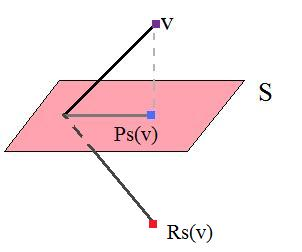
\includegraphics[scale=0.5]{proyeccion}\caption{Proyección y reflexión}
		\end{center}
	\end{figure}
\end{minipage}

\subsection{Matriz de Householder}
\begin{tikzpicture}
	\node [definicion] (box){%
		\begin{minipage}{0.80\textwidth}
			La matriz de reflexión sobre un subespacio de dimensión $n-1$ que es ortogonal a un vector $\vect{w}$ en un espacio de dimensión $n$ se puede obtener mediante la expresión:
			\begin{align}
				H=I_d-2\frac{\vect{w} \cdot \vect{w}^T}{\vect{w}^T \cdot \vect{w}}
			\end{align}
			Dicha matriz tiene las siguientes propiedades:
			\begin{itemize}
				\item Es involutiva: $H \circ H=I_d$
				\item Es simétrica: $H^T=H$
				\item Es inversible: $\exists H^{-1}$ y $\exists H^{-1}=H$
				\item Es ortogonal: $H^T H=H H^T=I_d$
			\end{itemize}
		\end{minipage}};
	\node[fancytitle, right=10pt] at (box.north west) {Propiedades de la proyección};
	\node[fancytitle, rounded corners] at (box.south) {$\aleph$};
\end{tikzpicture}

\subsection{Rotaciones en $R^3$}
\begin{tikzpicture}
	\node [definicion] (box){%
		\begin{minipage}{0.80\textwidth}
			Sea $B=\{\vect{v}_1,\vect{v}_2,\vect{v}_3 \}$ una Base Ortonormal (BON) de $R^3$ y sea $T$ la rotación $\theta$ grados alrededor del eje $v_i$:
			\begin{align}
				\text{Rotación sobre } \vect{v}_1 :[T]_B=\begin{bmatrix} {1}&{0}&{0} \\ {0}&{\cos (\theta)}&{-\sin(\theta)} \\ {0}&{\sin (\theta)}&{\cos (\theta)} \end{bmatrix} \\
				\text{Rotación sobre } \vect{v}_2 :[T]_B=\begin{bmatrix} {\cos (\theta)}&{0}&{-\sin(\theta)} \\ {0}&{1}&{0} \\ {\sin (\theta)}&{0}&{\cos (\theta)} \end{bmatrix} \\
				\text{Rotación sobre } \vect{v}_3 :[T]_B=\begin{bmatrix} {\cos (\theta)}&{-\sin(\theta)}&{0} \\ {\sin (\theta)}&{\cos (\theta)}&{0} \\ {0}&{0}&{1} \end{bmatrix} \\
			\end{align}
		\end{minipage}};
	\node[fancytitle, right=10pt] at (box.north west) {Rotaciones en $R^3$};
	\node[fancytitle, rounded corners] at (box.south) {$\aleph$};
\end{tikzpicture}

\subsection{Proceso de Gram-Schmidt}
\begin{tikzpicture}
	\node [definicion] (box){%
		\begin{minipage}{0.80\textwidth}
			Dada una base $\{\vect{x}_1,\vect{x}_2,\ldots,\vect{x}_p\}$ para un subespacio $W \in R^n$ defina:
			\begin{enumerate}
				\item $\vect{v}_1=\vect{x}_1$
				\item $\vect{v}_2=\vect{x}_2-\frac{\vect{x}_2 \cdot \vect{v}_1}{\vect{v}_1 \cdot \vect{v}_1}\vect{v}_1$
				\item $\vect{v}_p=\vect{x}_p-\sum_{i=1}^{p-1} \frac{\vect{x}_p \cdot \vect{v}_i}{\vect{v}_i \cdot \vect{v}_i}\vect{v}_i$
			\end{enumerate}
			Entonces $\{ \vect{v}_1,\vect{v}_2,\ldots,\vect{v}_p \}$ es una Base Ortogonal (BOG) de $W$.\\
			
			Si luego se divde a cada componente por la norma de la base se obtiene una Base Ortogonal (BON) de $W$.
		\end{minipage}};
	\node[fancytitle, right=10pt] at (box.north west) {Proceso de Gram-Schmidt};
	\node[fancytitle, rounded corners] at (box.south) {$\aleph$};
\end{tikzpicture}

\subsection{Matrices de proyección}
\begin{tikzpicture}
	\node [definicion] (box){%
		\begin{minipage}{0.80\textwidth}
			Utilizando el producto interno canónico de sobre $K^n$, con $K=R$ o $K=C$.\\
			
			$P \in K^{n \times n}$ es una matriz de proyección si y solo si:
			\begin{align}
				P^2=P \\
				P^H=P
			\end{align}
			Dicha matriz tiene las siguientes propiedades:
			\begin{itemize}
				\item $\col{P}=\nul{P}^\bot$
				\item $P \cdot y=y \Longleftrightarrow y \in \col{P}$
				\item Si $P_S$ es matriz de proyección sobre $S$ y $P_S^\bot$ es matriz de proyección sobre $S^\bot$ entonces $P_S+P_S^\bot=I_d$
				\item Las columnas de $P$ son una base del espacio sobre el cual proyectan
				\item $\rg{P}=\tr{P}$
				\item $\det{P} \neq 0$ si $P\neq I_d$
				\item Si $P_1$ y $P_2$ son matrices de proyección y $P_1 \cdot P_2=P_2 \cdot P_1=0$, entonces $P_1+P_2$ es matriz de proyección y $\rg{P_1+P_2}=\rg{P_1}+\rg{P_2}$
			\end{itemize}
			Obtención de la matriz de proyección:
			\begin{enumerate}
				\item Sea $Q$ una matriz cuyas columnas son una Base Ortonormal (BON) de $S \subset V$. Entonces la única matriz de proyección sobre $S$ es $[P_S]=Q \cdot Q^T$. La matriz de proyección sobre $S^\bot$ es $[P_S^\bot]=I_d-[P_S]$
				\item Sea $B=\{\vect{v}_1,\ldots,\vect{v}_q \}$ una base de $S$, y $A$ la matriz que tiene por columnas a $\vect{v}_1,\ldots,\vect{v}_q$. Entonces la única matriz de proyección sobre $S$ se obtiene mediante $[P_S]=A\left(A^H A\right)^{-1} A^H=A A^{\#}$
				\end{enumerate}
		\end{minipage}};
	\node[fancytitle, right=10pt] at (box.north west) {Matriz de proyección};
	\node[fancytitle, rounded corners] at (box.south) {$\aleph$};
\end{tikzpicture}

\subsection{Inversas y pseudoinversas}
\begin{tikzpicture}
	\node [definicion] (box){%
		\begin{minipage}{0.80\textwidth}
			Sea $A \in K^{n \times q} \vert \rg{A}=q$. La matriz pseudoinversa de $A$ es $A^{\#}=\left(A^H A\right)^{-1} A^H$:
			\begin{itemize}
				\item Si $A$ es cuadrada invertible, $A^{-1}=A^{\#}$
				\item $A^{\#} \in R^{q \times n}$
				\item $A^{\#}A=I_{d_{(q)}}$
				\item $A A^{\#}=[P]_{\col{A}}$
				\item $\nul{A A^{\#}}=[\col{A}]^\bot$ 
			\end{itemize}
		\end{minipage}};
	\node[fancytitle, right=10pt] at (box.north west) {Propiedades de la pseudoinversa};
	\node[fancytitle, rounded corners] at (box.south) {$\aleph$};
\end{tikzpicture}

\subsection{Cuadrados mínimos}
\begin{tikzpicture}
	\node [definicion] (box){%
		\begin{minipage}{0.80\textwidth}
			Sea $A \in K^{n \times q}, \vect{x} \in K^q, \vect{b} \in R^n$. Si $Ax=b$ tiene una solución extra, entonces $\vect{b} \in \col{A}$. Si $b \notin \col{A}$, intentamos hallar una solución $\hat{\vect{x}} \in K^q$ (la solución por \textbf{cuadrados mínimos}) tal que:
			\begin{minipage}{0.65\textwidth}
				\begin{itemize}
					\item $\dete{A\hat{\vect{x}}-\vect{b}} < \dete{A\vect{u}-\vect{b}}$, $\forall \vect{u} \in K^q$	
					\item $d(A\hat{\vect{x}},\vect{b}) \leq d(A\vect{u},\vect{b})$, $ \forall \vect{u} \in K^q$
					\item $\dete{A\hat{\vect{x}}} \leq \dete{\vect{b}}$ (Son iguales si $\vect{b} \in \col{A}$)
					\item Ecuaciones normales de cuadrados mínimos: $A^T A \hat{\vect{x}}=A^T \vect{b}=\hat{\vect{b}}$
					\item $A \hat{\vect{x}}=\hat{\vect{b}}=P_{\col{A}}(\vect{b})$ si y solo si:
						\begin{align}
							A\hat{\vect{x}} \in \col{A} \\
							\vect{b}-A\hat{\vect{x}} \in \col{A}^\bot
						\end{align}
				\end{itemize}
			\end{minipage}
			\begin{minipage}{0.3\textwidth}
				\begin{figure}[H]
					\begin{flushright}
						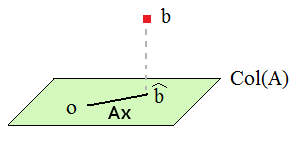
\includegraphics[scale=0.35]{cuad_min}\caption{Cuadrados mínimos}
					\end{flushright}
				\end{figure}
			\end{minipage}
		\end{minipage}};
	\node[fancytitle, right=10pt] at (box.north west) {Cuadrados mínimos};
	\node[fancytitle, rounded corners] at (box.south) {$\aleph$};
\end{tikzpicture}

\begin{tikzpicture}
	\node [corolario] (box){%
		\begin{minipage}{0.80\textwidth}
			\begin{enumerate}
				\item Si $\hat{\vect{x}}=0$ entonces $\vect{b} \in [\col{A}]^\bot$. La recíproca solo es cierta si $A$ es invertible.
				\item Si las columnas de $A$ son linealmente independientes, la solución por cuadrados mínimos es única y se obtiene mediante:
					\begin{align}
						\hat{\vect{x}}=(A^T A)^{-1}A^T \vect{b}=A^{\#}\vect{b}
					\end{align}
				Si las columnas de $A$ son linealmente dependientes, el sistema $A^T A\hat{\vect{x}}=A^T b$ tiene infinitas soluciones, y éstas son de la forma $\hat{\vect{x}}=\hat{\vect{x}}_p+\underbrace{\hat{\vect{x}}_n}_{\in \nul{A}}$
				\item Si $\vect{b} \in \col{A}$, entonces toda solución de $A\vect{x}=\vect{b}$ es una solución exacta y por cuadrados mínimos
				\item El error de aproximación $\epsilon$ es igual a $\dete{\vect{b}-\hat{\vect{b}}}$
			\end{enumerate}
		\end{minipage}};
	\node[fancytitle, right=10pt] at (box.north west) {Propiedades de Cuadrados mínimos};
	\node[fancytitle, rounded corners] at (box.south) {$\aleph$};
\end{tikzpicture}

\subsubsection{Norma mínima}
\begin{tikzpicture}
	\node [corolario] (box){%
		\begin{minipage}{0.80\textwidth}
			La solución por cuadrados mínimos de norma mínima pertenece al espacio $\fil{A}$y se obtiene como:
			\begin{align}
				\tilde{\vect{x}}=A^+ \vect{b}
			\end{align}
			Siendo $A^+$ la \textbf{pseudoinversa de Moore-Penrose} de $A$.
		\end{minipage}};
	\node[fancytitle, right=10pt] at (box.north west) {Pseudoinversa de Moore-Pensore};
	\node[fancytitle, rounded corners] at (box.south) {$\aleph$};
\end{tikzpicture}

\subsection{Regresión lineal}
\begin{tikzpicture}
	\node [definicion] (box){%
		\begin{minipage}{0.80\textwidth}
			Sean los puntos $\vect{P}_i=(x_i,y_i)$ con $i=1,2,\ldots,n$. La recta que mejor aproxima a los puntos es:
			\begin{align}
				\vect{y}=\alpha_0\vect{1}+\alpha_1 \vect{x}
			\end{align}
			Y los coeficientes $\alpha_i$ se obtienen resolviendo el sistema:
			\begin{align}
				\begin{bmatrix}{1}&{x_1}\\{1}&{x_2}\\{\vdots}&{\vdots} \\{1}&{x_n} \end{bmatrix} \begin{bmatrix}{\alpha_0}\\{\alpha_1}\end{bmatrix}=\begin{bmatrix}{y_1}\\{y_2}\\{\vdots}\\{y_n}\end{bmatrix}
			\end{align}
			Si se aproxima por una parábola se agrega otro nivel de complejidad, con $y=\alpha_2x^2+\alpha_1x+\alpha_0$, lo que implica una columna adicional a la matriz para los términos cuadráticos, una fila adicional para la constante $\alpha_2$ en la variable.\\
			
			Se siguen agregando columnas a la matriz y filas al vector tantas veces como grados de complejidad se necesiten.
		\end{minipage}};
	\node[fancytitle, right=10pt] at (box.north west) {Regresión lineal};
	\node[fancytitle, rounded corners] at (box.south) {$\aleph$};
\end{tikzpicture}

\newpage
\section{Transformaciones lineales}
Sea $T \in \ell (V_K,W_K)$ y $A=[T]_{BC}$ con $B$ base de $V$ y $C$ base de $W$ la matriz de $T$.

\subsection{Condiciones para las Transformaciones lineales}
\begin{tikzpicture}
	\node [definicion] (box){%
		\begin{minipage}{0.80\textwidth}
			Para que una transformación se considere lineal debe cumplir:
			\begin{enumerate}
				\item $T(\vect{u}+\vect{v})=T(\vect{u})+T(\vect{v})$, con $\vect{u},\vect{v}$ $\in V$
				\item $T(\alpha \vect{u}+\beta \vect{v})=\alpha \cdot T(\vect{u})+\beta \cdot T(\vect{v})$, con $\vect{u},\vect{v} \in V_K$ y $\alpha,\beta \in K$
				\item $T(0_{V_K})=0_{V_K}$
			\end{enumerate}
		\end{minipage}};
	\node[fancytitle, right=10pt] at (box.north west) {Condiciones para ser Transformación lineal};
	\node[fancytitle, rounded corners] at (box.south) {$\aleph$};
\end{tikzpicture}

\subsection{Núcleo e Imágen}
\begin{tikzpicture}
	\node [definicion] (box){%
		\begin{minipage}{0.80\textwidth}
			\textbf{Núcleo:} $\nul{T}=\{ \vect{v} \in V_K \text{ } \vert \text{ } T(\vect{v})=0_W \}=C_B^{-1}(\nul{A})$.\\
			\textbf{Imágen:} $\im{T}=\{ \vect{w} \in W_K \text{ } \vert \text{ } T(\vect{v})=\vect{w} \text{ con } \vect{v} \in V_K \}=C_C^{-1}(\col{A})$.\\
			
			Ambos son subespacios vectoriales.\\
			
			La imágen de una Transformación Lineal puede obtenerse como lo que generan los transformados de una base del espacio de partida.
		\end{minipage}};
	\node[fancytitle, right=10pt] at (box.north west) {Núcleo e Imágen};
	\node[fancytitle, rounded corners] at (box.south) {$\aleph$};
\end{tikzpicture}

\begin{tikzpicture}
	\node [teorema] (box){%
		\begin{minipage}{0.80\textwidth}
			Sea $T \in \ell (V,W)$ y sea $\dime{V}=n$ (finita). Entonces:
			\begin{align}
				\dime{V}=\dime{\nul{T}}+\dime{\im{T}}
			\end{align}
		\end{minipage}};
	\node[fancytitle, right=10pt] at (box.north west) {Teorema de la dimensión};
	\node[fancytitle, rounded corners] at (box.south) {$\aleph$};
\end{tikzpicture}

\subsection{Clasificación de las Transformaciones lineales}
\subsubsection{Monomorfismo(Inyectividad)}
\begin{tikzpicture}
	\node [definicion] (box){%
		\begin{minipage}{0.80\textwidth}
			Una Transformación lineal es inyectiva si verifica:
			\begin{align}
				\vect{v}_1 \neq \vect{v}_2 \Rightarrow T(\vect{v}_1) \neq T(\vect{v}_2) \text{ , } \forall \vect{v}_1,\vect{v}_2 \in V \\
				\nul{T}=\{0_V\} \Longleftrightarrow \dime{\im{T}}=\dime{V}
			\end{align}
			Una Transformación Lineal Inyectiva transforma conjuntos Linealmente Independientes a conjuntos Linealmente Independientes.\\
			
			La recíproca también es cierta: si $A$ es un conjunto Linealmente Independiente y es transformado en otro conjunto Linealmente Independiente, la Transformación Lineal es inyectiva. Es decir: Si $T$ es inyectiva y $A$ es Linealmente Independiente, $T(A)$ es Linealmente Independiente.\\
			
			Las matrices asociadas a Transformaciones Lineales inyectivas tienen sus columnas Linealmente Independientes.\\
			
			Si $\dime{V} > \dime{W}$, $T$ \underline{no} puede ser inyectiva.
		\end{minipage}};
	\node[fancytitle, right=10pt] at (box.north west) {Monomorfismo};
	\node[fancytitle, rounded corners] at (box.south) {$\aleph$};
\end{tikzpicture}

\subsubsection{Epimorfismo(Sobreyectividad)}
\begin{tikzpicture}
	\node [definicion] (box){%
		\begin{minipage}{0.80\textwidth}
			Una Transformación lineal es sobreyectiva si y solo si:
			\begin{align}
				\im{T}=W
			\end{align}
			Las matrices asociadas a Transformaciones lineales sobreyectivas tienen sus filas Linealmente Independientes.\\
			
			Si $\dime{W} > \dime{V}$, $T$ \underline{no} puede ser sobreyectiva.
		\end{minipage}};
	\node[fancytitle, right=10pt] at (box.north west) {Epimorfismo};
	\node[fancytitle, rounded corners] at (box.south) {$\aleph$};
\end{tikzpicture}

\subsubsection{Isomorfismo(Biyectividad)}
\begin{tikzpicture}
	\node [definicion] (box){%
		\begin{minipage}{0.80\textwidth}
			Una Transformación lineal es biyectiva si y solo si:
			\begin{align}
				\dime{W}=\dime{V} \\
				\nul{T}=\{ 0_V \}
			\end{align}
			Es decir, si es Inyectiva y Sobreyectiva a la vez.\\
			
			$T$ es biyectiva $\Longleftrightarrow$ si $\{\vect{v}_1,\ldots,\vect{v}_n \}$ es base de $V$ $\Rightarrow$ $\{T(\vect{v}_1),\ldots,T(\vect{v}_n) \}$ es base de $W$\\
			La matriz asociada a una Transformación lineal biyectiva tiene sus filas y columnas Linealmente Independientes, o sea que es una matriz inversible, es decir, existe una transformación lineal inversa $T^{-1}=[T]^{-1}$\\
			
			Si $\dime{V}=\dime{W}$, entonces o bien $T$ es inyectiva y sobreyectiva, o no es ninguna de las dos.
		\end{minipage}};
		\node[fancytitle, right=10pt] at (box.north west) {Biyectividad};
		\node[fancytitle, rounded corners] at (box.south) {$\aleph$};
	\end{tikzpicture}

\subsection{Matriz asociada a una Transformación lineal}
\begin{tikzpicture}
	\node [definicion] (box){%
		\begin{minipage}{0.80\textwidth}
			Sea $T \in \ell (V_K,W_K)$, sea $B=\{ \vect{v}_1,\ldots,\vect{v}_q \}$ base de $V$ y $C=\{ \vect{w}_1,\ldots,\vect{w}_m \}$ base de $W$. Entonces $T$ se puede escribir como $T(\vect{x})=A\vect{x}$, con $A \in K^{m \times q}$ tal que:
			\begin{align}
				A=[T]_{BC}=\begin{bmatrix}{|}&{|}&{ }&{|}\\{C_C(T(\vect{v}_1))}&{C_C(T(\vect{v}_2))}&{\ldots}&{C_C(T(\vect{v}_q))}\\{|}&{|}&{ }&{|}\end{bmatrix}
			\end{align}
			Dicha matriz posee las siguientes propiedades:
			\begin{itemize}
				\item $[T]_{BC} \cdot C_B(\vect{v})=C_C(T(\vect{v}))$ $,\forall \vect{v} \in V$
				\item $\vect{v} \in \nul{T} \Longleftrightarrow C_B(\vect{v}) \in \nul{A}$
				\item $\vect{w} \in \im{T} \Longleftrightarrow C_C(\vect{w}) \in \col{A}$
				\item $\dime{\im{T}}=\rg{A}$
			\end{itemize}
		\end{minipage}};
	\node[fancytitle, right=10pt] at (box.north west) {Matriz de la Transformación lineal};
	\node[fancytitle, rounded corners] at (box.south) {$\aleph$};
\end{tikzpicture}

\begin{tikzpicture}
	\node [teorema] (box){%
		\begin{minipage}{0.80\textwidth}
			Sean $V$y $W$ $K$-espacios vectoriales ($K=R$ o $C$). Sea $T:V \to W$.\\
			
			Si $B_1$ y $B_2$ son bases ordenadas de $V$, y $C_1$ y $C_2$ son bases ordenadas de $W$, entonces:
			\begin{align}
				\rg{[T]_{B_1 C_1}}=\rg{[T]_{B_2 C_2}}
			\end{align}
		\end{minipage}};
	\node[fancytitle, right=10pt] at (box.north west) {Teorema para matrices de Transformación lineal};
	\node[fancytitle, rounded corners] at (box.south) {$\aleph$};
\end{tikzpicture}

\subsection{Teorema fundamental de las Transformaciones lineales}
\begin{tikzpicture}
	\node [teorema] (box){%
		\begin{minipage}{0.80\textwidth}
			Sea $B=\{\vect{v}_1,\ldots,\vect{v}_n \}$ base de $V$ y $\vect{w}_1,\ldots,\vect{w}_n$ vectores de $W$. Entonces existe y es única la Transformación lineal que verifica:
			\begin{align}
				T(\vect{v}_i)=\vect{w}_i \text{ , } \forall i=1,\ldots,n
			\end{align}
			Además, dada una Transformación lineal y un par de bases, existe una única matriz asociada.\\
			
			La recíproca tambíen es verdadera: dada una matriz y un par de bases, existe una única Transformación lineal asociada.
		\end{minipage}};
	\node[fancytitle, right=10pt] at (box.north west) {Teorema fundamental de las Transformaciones lineales};
	\node[fancytitle, rounded corners] at (box.south) {$\aleph$};
\end{tikzpicture}

\subsection{Composición de Transformaciones lineales}
\begin{minipage}{0.6\textwidth}
	\begin{tikzpicture}
		\node [definicion] (box){%
			\begin{minipage}{0.90\textwidth}
				Sea $f \in \ell (V,W)$ y $g \in \ell (W,H)$ $\Rightarrow g \circ f \in (V,H)$. Podemos encontrar la siguientes propiedades:
				\begin{align}
					\nul{f} \subseteq \nul{g \circ f} \\
					\im{g \circ f} \subseteq \im{g}
				\end{align}
			\end{minipage}};
		\node[fancytitle, right=10pt] at (box.north west) {Composición de Transformaciones lineales};
		\node[fancytitle, rounded corners] at (box.south) {$\aleph$};
	\end{tikzpicture}
\end{minipage}
\begin{minipage}{0.3\textwidth}
	\begin{figure}[H]
		\begin{center}
			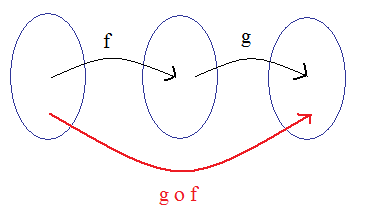
\includegraphics[scale=0.3]{composicion}\caption{Composición}
		\end{center}
	\end{figure}
\end{minipage}

\subsection{Operadores lineales}
\begin{tikzpicture}
	\node [definicion] (box){%
		\begin{minipage}{0.80\textwidth}
			Un operador lineal es una Transformación lineal que va de un espacio en si mismo, se escríbe como $T \in \ell (V)$ y cuenta con las siguientes propiedades:
			\begin{itemize}
				\item Si $T_1 \in \ell (V)$ y $T_2 \in \ell (V)$, entonces $T_1 \circ T_2 \in \ell (V)$
				\item Si $T \in \ell (V)$, $T^n=\underbrace{T \circ T \circ \ldots \circ T}_{\text{n veces}}$
			\end{itemize}
		\end{minipage}};
	\node[fancytitle, right=10pt] at (box.north west) {Operadores lineales};
	\node[fancytitle, rounded corners] at (box.south) {$\aleph$};
\end{tikzpicture}

\newpage
\section{Autovalores y Autovectores}
\subsection{Definiciones básicas}
\begin{tikzpicture}
	\node [definicion] (box){%
		\begin{minipage}{0.80\textwidth}
			\textbf{Autovector:} Un vector $\vect{v} \neq 0$ es autovector de $A \in K^{n \times n} \Longleftrightarrow \exists \lambda \in K$ $\vert$ $A \vect{v}=\lambda \vect{v}$\\
			
			\textbf{Autoespacio:} El autoespacio de $A$ asociado a un autovalor $\lambda$ es $S_\lambda (A)=\nul{A-\lambda I}$\\
			
			\textbf{Polinomio característico:} El polinomio característico de una matriz $A \in K^{n \times n}$ es $p_A(\lambda)=\dete{A-\lambda I}$, y tiene grado $n$. Si $K=R$ el polinomio tiene a lo sumo $n$ raíces. Si $K=C$ tiene exactamente $n$ raíces.\\
			
			\textbf{Autovalor:} Los autovalores $\lambda$ de una matriz son las raíces de su polinomio característico.\\
			
			\textbf{Espectro de una matriz:} $\sigma (A)=\{ \lambda \in K$ $\vert$ $\lambda$ es autovalor de $A \}$.
		\end{minipage}};
	\node[fancytitle, right=10pt] at (box.north west) {Definiciones básicas};
	\node[fancytitle, rounded corners] at (box.south) {$\aleph$};
\end{tikzpicture}

\subsection{Autovalores complejos de matriz real}
\begin{tikzpicture}
	\node [definicion] (box){%
		\begin{minipage}{0.80\textwidth}
			Supongamos que $\vect{v}$ es un autovector de $A \in R^{n \times n}$ asociado a $\lambda=a+\jmath b$ con $a,b \in R,b \neq 0$.\\
			Entonces $\vect{v}^*$ es también un autovector de $A \in R^{n \times n}$ asociado a $\lambda^*=a-\jmath b$.\\
			
			En particular si $\{\vect{v}_1,\ldots,\vect{v}_n \}$ es una base de $S_\lambda$, entonces $\{\vect{v}_1^*,\ldots,\vect{v}_n^* \}$ es una base de $S_{\lambda^*}$
		\end{minipage}};
	\node[fancytitle, right=10pt] at (box.north west) {Autovalores complejos};
	\node[fancytitle, rounded corners] at (box.south) {$\aleph$};
\end{tikzpicture}

\subsection{Multiplicidad geométrica y algebráica de un Autovalor}
\begin{tikzpicture}
	\node [definicion] (box){%
		\begin{minipage}{0.80\textwidth}
			Se define:
			\begin{itemize}
				\item $m_g(\lambda)=\dime{S_\lambda(A)}$
				\item $m_a(\lambda) \doteq$ número de veces que aparece $\lambda$ como raíz del polinomio característico.
			\end{itemize}
			
			Siempre se verifica que:
			\begin{align}
				1 \leq m_g(\lambda) \leq m_a(\lambda)
			\end{align}
		\end{minipage}};
	\node[fancytitle, right=10pt] at (box.north west) {Multiplicidad de Autovalores};
	\node[fancytitle, rounded corners] at (box.south) {$\aleph$};
\end{tikzpicture}

\subsection{Propiedades}
\begin{tikzpicture}
	\node [definicion] (box){%
		\begin{minipage}{0.80\textwidth}
			Sea $A \in K^{n \times n}$:
			\begin{itemize}
				\item $A$ es singular $\Longleftrightarrow 0$ es un autovalor de $A \Longleftrightarrow m_g(0)=n-k \Longleftrightarrow \rg{A}=k<n$
				\item Dos autovectores asociados a autovalores distintos son Linealmente Independientes
				\item Si $A \in K^{2x2}$, entonces $p_A(\lambda)=\lambda^2-\tr{A}\lambda+\dete{A}$
				\item Si todas las filas o columnas de $A$ sumas $s$, entonces $s$ es autovalor de $A$.
				\item Sea $p(t)$ un polinomio de grado $k$. Si $\lambda$ es autovalor de $A$, entonces se cumple que $p(\lambda)$ es autovalor de $p(A)$, y para cada autovalor $\mu$ de $p(A)$ existe un autovalor $\lambda$ de $A$ tal que $p(\lambda)=\mu$.
				\item Si $\lambda$ es autovalor de $A$:
				\begin{itemize}
					\item $\lambda$ es autovalor de $A^T$
					\item $\lambda^{-1}$ es autovalor de $A^{-1}$ y $S_{\lambda^{-1}}\left(A^{-1}\right)=S_\lambda(A)$
					\item $r \cdot \lambda$ es autovalor de $r \cdot A$
					\item $\lambda^k$ es autovalor de $A^k$, con $k \in N$
					\item $\lambda+r$ es autovalor de $A+r \cdot I$
				\end{itemize}
			\end{itemize}
		\end{minipage}};
	\node[fancytitle, right=10pt] at (box.north west) {Propiedades de Autovalores y Autovectores};
	\node[fancytitle, rounded corners] at (box.south) {$\aleph$};
\end{tikzpicture}

\subsection{Autovalores y Autovectores de operadores lineales}
\begin{tikzpicture}
	\node [definicion] (box){%
		\begin{minipage}{0.80\textwidth}
			$T:V_K \to V_K$. Un vector $\vect{v} \neq \vect{0}$ es autovector de $T \Longleftrightarrow T(\vect{v})=\lambda \vect{v}$, con $\lambda$ autovalor de $T$.\\
			$S_\lambda(T)=\{ \vect{x} \in V$ $\vert$ $T(\vect{x})=\lambda \vect{x}$ y $\lambda$ autovalor de $T\}=\nul{T-\lambda I}$. Si $B$ es base de $V$ y $A$ es la matriz de $T$ en esa base, entonces:
			\begin{align}
				\sigma(A)=\sigma(T) \forall B \text{ base de } V \\
				\vect{x} \text{ es autovector de } T \Longleftrightarrow C_B(\vect{x}) \text{ es autovector de } [T]_B=A
			\end{align}
			Se deducen las siguientes propiedades:
			\begin{itemize}
				\item $T(\vect{x})=\lambda \vect{x} \Rightarrow T^n(\vect{x})=\lambda^n \vect{x}$, $n \in N$
				\item Si $\lambda$ es autovalor de $T$, $\lambda^{-1}$ es autovalor de $T^{-1}$
				\item Si $h$ es un polinomio en $K$ y $T(\vect{x})=A\vect{x}$, entonces:
				\begin{align}
					\sigma[h(A)]=h[\sigma(A)] \\
					S_{h(\lambda)}h(A)=S_\lambda(A)
				\end{align}
				\item $T:V_K \to V_K$ es regular $\Longleftrightarrow 0 \notin \sigma(T)$
			\end{itemize}
		\end{minipage}};
	\node[fancytitle, right=10pt] at (box.north west) {Autovalores y Autovectores de Operadores lineales};
	\node[fancytitle, rounded corners] at (box.south) {$\aleph$};
\end{tikzpicture}

\subsection{Diagonalización}
\begin{tikzpicture}
	\node [definicion] (box){%
		\begin{minipage}{0.80\textwidth}
			Los siguientes enunciados son equivalentes para definir si $A \in K^{n \times n}$ es diagonalizable:
			\begin{itemize}
				\item $A \sim D$
				\item $\exists$ una base de $K^n$ compuesta por autovectores de $A$
				\item $A$ tiene $n$ autovalores Linealmente Independientes 
				\item $m_g(\lambda)=m_a(\lambda)$ $\forall \lambda \in \sigma(A)$
				\item $\exists P$ invertible y $D$ diagonal tal que:
				\begin{align}
					A=PDP^{-1}
				\end{align}
				Siendo $P$ la matriz de autovectores y $D$ la matriz diagonal de autovalores.
			\end{itemize}
		\end{minipage}};
	\node[fancytitle, right=10pt] at (box.north west) {Diagonalización};
	\node[fancytitle, rounded corners] at (box.south) {$\aleph$};
\end{tikzpicture}

\subsubsection{Matrices trivialmente diagonalizables}
\begin{tikzpicture}
	\node [definicion] (box){%
		\begin{minipage}{0.80\textwidth}
			\begin{itemize}
				\item \textbf{Matriz nula:}
					\begin{itemize}
						\item \textbf{Autovalores:} 0
						\item \textbf{Autovectores:} Cualquier vector no nulo
					\end{itemize}
				\item \textbf{Matriz identidad:}
					\begin{itemize}
						\item \textbf{Autovalores:} 1
						\item \textbf{Autovectores:} Cualquier vector no nulo
					\end{itemize}
				\item \textbf{Matriz diagonal:}
					\begin{itemize}
						\item \textbf{Autovalores:} $a_{ii}$, los elementos de la diagonal
						\item \textbf{Autovectores:} Los que tienen sus componentes nulas, excepto la $n$-ésima.
					\end{itemize}
				\item \textbf{Matriz escalar:}
					\begin{itemize}
						\item \textbf{Autovalores:} $k \in R$
						\item \textbf{Autovectores:} Cualquier vector no nulo
					\end{itemize}
				\item \textbf{Matriz de proyección:}
					\begin{itemize}
						\item \textbf{Autovalores:} 1 con $m_a(1)=m_g(1)=\dime{S}$ y 0 con $m_a(0)=m_g(0)=\dime{S^\bot}$
						\item \textbf{Autovectores:} Los vectores de $S$ asociados a 1 y los asociados a $S^\bot$ a 0
					\end{itemize}
				\item \textbf{Matriz de reflexión:}
					\begin{itemize}
						\item \textbf{Autovalores:} 1 con $m_a(1)=m_g(1)=\dime{S}$ y -1 con $m_a(-1)=m_g(-1)=\dime{S^\bot}$
						\item \textbf{Autovectores:} Los vectores de $S$ asociados a 1 y los asociados a $S^\bot$ a -1
					\end{itemize}
			\end{itemize}
		\end{minipage}};
	\node[fancytitle, right=10pt] at (box.north west) {Diagonalizaciones triviales};
	\node[fancytitle, rounded corners] at (box.south) {$\aleph$};
\end{tikzpicture}

\subsubsection{Propiedades}
\begin{tikzpicture}
	\node [definicion] (box){%
		\begin{minipage}{0.80\textwidth}
			\begin{itemize}
				\item Si $A$ es diagonalizable entonces $A^n$ es diagonalizable ($D_A^n=D_{A^n}$ y $\sigma(A^n)=\sigma^n(A)$). La recíproca es falsa
				\item Si $A \in C^{n \times n}$ tiene $n$ autovalores distintos entonces $A$ es diagonalizable. La recíproca es falsa
				\item $\dete{A}=\prod_{i=1}^n \lambda_i=p_A(0)$
				\item $\tr{A}=\sum_{i=1}^n \lambda_i$
			\end{itemize}
		\end{minipage}};
	\node[fancytitle, right=10pt] at (box.north west) {Propiedades de la diagonalización};
	\node[fancytitle, rounded corners] at (box.south) {$\aleph$};
\end{tikzpicture}

\subsubsection{Diagonalización de transformaciones lineales}
\begin{tikzpicture}
	\node [definicion] (box){%
		\begin{minipage}{0.80\textwidth}
			Los siguientes enunciados son equivalentes para decir que $T \in \ell (V_K)$ con $\dime{V_K}=n$, es diagonalizable:
			\begin{itemize}
				\item $\exists B$ base de $V_K$ tal que $[T]_B$ es diagonal
				\item $\exists B$ base de $V_K$ formada por autovectores de $T$
				\item $T$ tiene $n$ autovectores Linealmente Independientes 
			\end{itemize}
			Esa base $B$ y $[T]_B=\text{diag}(\sigma(T))$.\\
			
			Si $A=[T]_H$, $H$ cualquiera base, entonces $T$ es diagonalizable si y solo si $A$ es diagonalizable.
		\end{minipage}};
	\node[fancytitle, right=10pt] at (box.north west) {Diagonalización de Transformaciones Lineales};
	\node[fancytitle, rounded corners] at (box.south) {$\aleph$};
\end{tikzpicture}

\newpage
\section{Matrices hermíticas y simétricas}
\subsection{Diagonalización}
\begin{tikzpicture}
	\node [definicion] (box){%
		\begin{minipage}{0.80\textwidth}
			\textbf{Matriz antisimétrica:} Si $A \in R^{n \times n}$ es antisimétrica ($A^T=A$) entonces:
			\begin{itemize}
				\item Los autovalores de $A$ son imaginarios puros o nulos
				\item Los autovectores asociados a autovalores distintos son ortogonales
				\item $A$ es diagonalizable unitariamente.
			\end{itemize}
		\end{minipage}};
	\node[fancytitle, right=10pt] at (box.north west) {Matriz antisimétrica};
	\node[fancytitle, rounded corners] at (box.south) {$\aleph$};
\end{tikzpicture}

\begin{tikzpicture}
	\node [definicion] (box){%
		\begin{minipage}{0.80\textwidth}
			\textbf{Matriz simétrica(hermítica):} Si $A \in R^{n \times n}$ es simétrica ($B \in C^{n \times n}$ es hermítica) si y solo si:\\
			$A$ es diagonalizable ortogonalmente:
				\begin{align}
					A=PDP^T
				\end{align}
			$B$ es diagonalizable unitariamente:
				\begin{align}
					B=PDP^H
				\end{align}
			Con $D$ real.\\
			
			Se deducen las siguientes propiedades:
			\begin{itemize}
				\item $A$ y $B$ tienen $n$ autovalores reales
				\item Los elementos de la diagonal de $A$ y $B$ son reales
				\item $\dete{A} \in R$
				\item $\dime{S_\lambda(A)}=m_a(\lambda) \forall \lambda \in \sigma(A)$
				\item $\dime{S_\lambda(B)}=m_a(\lambda) \forall \lambda \in \sigma(B)$
				\item Los autovectores asociados a autovalores distintos son ortogonales
			\end{itemize}
		\end{minipage}};
	\node[fancytitle, right=10pt] at (box.north west) {Matriz simétrica(hermítica)};
	\node[fancytitle, rounded corners] at (box.south) {$\aleph$};
\end{tikzpicture}

\begin{tikzpicture}
	\node [definicion] (box){%
		\begin{minipage}{0.80\textwidth}
			\textbf{Matriz ortogonal(unitaria):} Si $A \in R^{n \times n}$ es ortogonal ($B \in C^{n \times n}$ es unitaria) si y solo si:\\
			
			\begin{minipage}{0.4\textwidth}
				\begin{align}
					A A^T=A^T A=I_d \\
					A^T=A^{-1}
				\end{align}
			\end{minipage}
			\begin{minipage}{0.1\textwidth}
				\begin{flushright}
					ó
				\end{flushright}
			\end{minipage}
			\begin{minipage}{0.4\textwidth}
				\begin{align}
					B B^H=B^H B=I_d \\
					B^H=B^{-1}
				\end{align}
			\end{minipage}
			\vspace{0.5cm}
			Las columnas de $A$ y $B$ son Base Ortonormal de $R^n$ y $C^n$ respectivamente.\\
			
			Se deducen las siguientes propiedades:
			\begin{itemize}
				\item $\dete{A}=\pm 1$. Si $\dete{A}=1$, $A$ es la matriz de rotación
				\item Los autovalores tienen módulo $1$ y pueden ser reales o complejos
				\item Son matrices unitariamente diagonalizables
				\item Los autovectores asociados a autovalores distintos son ortogonales
				\item Preservan los productos internos: $\produ{A\vect{x},A\vect{y}}=\produ{\vect{x},\vect{y}}$
				\item Preservan las normas asociadas al producto interno: $\vert A \vect{x} \vert= \vert \vect{x} \vert$
				\item Si $C$ es unitaria, $BC$ y $CB$ son unitarias también.
			\end{itemize}
		\end{minipage}};
	\node[fancytitle, right=10pt] at (box.north west) {Matriz ortogonal(unitaria)};
	\node[fancytitle, rounded corners] at (box.south) {$\aleph$};
\end{tikzpicture}

\subsection{Descomposición espectral}
\begin{tikzpicture}
	\node [definicion] (box){%
		\begin{minipage}{0.80\textwidth}
			Si $A=PDP^{-1}=PDP^T$, las columnas de $P$ son autovectores ortonormales $\vect{u}_1,\ldots,\vect{u}_n$ de $A$ y los autovalores correspondientes $\lambda_1,\ldots,\lambda_n$ están en la matriz diagonal $D$. Entonces:
			\begin{align}
				A=\sum_{i=1}^n \lambda_i\vect{u}_i \vect{u}_i^T
			\end{align}
		\end{minipage}};
	\node[fancytitle, right=10pt] at (box.north west) {Descomposición espectral de matrices simétricas};
	\node[fancytitle, rounded corners] at (box.south) {$\aleph$};
\end{tikzpicture}

\subsection{Subespacios invariantes por una transformación lineal}
\begin{tikzpicture}
	\node [definicion] (box){%
		\begin{minipage}{0.80\textwidth}
			\begin{itemize}
				\item $S \in K^n$ es invariante por $A \in K^{n \times n} \Longleftrightarrow \forall \vect{x} \in S$ $\vert$ $A\vect{x} \in S$
				\item $S \subset V$ es invariante por $T \in \ell (V) \Longleftrightarrow \forall \vect{x} \in S$ $\vert$ $T(\vect{x}) \in S$
			\end{itemize}
			Se deducen las siguientes propiedades:
			\begin{itemize}
				\item Si $\lambda$ es autovalor de $T$, entonces $S_\lambda(T)$ es un subespacio invariante por $T$, puesto que:
				\begin{align}
					\forall \vect{x} \in S_\lambda(T) \Rightarrow T(\vect{x})=\lambda \vect{x} \in S_\lambda(T)
				\end{align}
				\item No todo subespacio invariante es un autoespacio de $T$, pero sí los de dimensión 1
			\end{itemize}
		\end{minipage}};
	\node[fancytitle, right=10pt] at (box.north west) {Subespacios invariantes por una transformación lineal};
	\node[fancytitle, rounded corners] at (box.south) {$\aleph$};
\end{tikzpicture}

\newpage
\section{Formas cuadráticas}
\begin{tikzpicture}
	\node [definicion] (box){%
		\begin{minipage}{0.80\textwidth}
			Una forma cuadrática en $R^n$ es una función $Q:R^n \to R$ tal que:
			\begin{align}
				Q(\vect{x})=\vect{x}^TA\vect{x}
			\end{align}
			 Donde $A$ es una matriz simétrica $\in R^{n \times n}$.
		\end{minipage}};
	\node[fancytitle, right=10pt] at (box.north west) {Formas cuadráticas};
	\node[fancytitle, rounded corners] at (box.south) {$\aleph$};
\end{tikzpicture}

\begin{tikzpicture}
	\node [teorema] (box){%
		\begin{minipage}{0.80\textwidth}
			Sea $A$ una matriz simétrica $\in R^{n \times n}$. Entonces existe un cambio ortogonal de variable, $\vect{x}=P\vect{y}$, donde $P$ es una matriz ortogonal tal que $\dete{P}=+1$ e $\vect{y}$ es el nuevo vector, que transforma la forma cuadrática $\vect{x}^TA\vect{x}$ a una forma cuadrática $\vect{y}^T D \vect{y}$ sin términos cruzados:
			\begin{align}
				\vect{x}^T A \vect{x}=\left(P\vect{y}\right)^T A \left(P\vect{y}\right)=\vect{y}^T \underbrace{P^T A P}_{D} \vect{y}=\vect{y}^T D \vect{y}=g(\vect{y})
			\end{align}
		\end{minipage}};
	\node[fancytitle, right=10pt] at (box.north west) {Teorema de los ejes principales};
	\node[fancytitle, rounded corners] at (box.south) {$\aleph$};
\end{tikzpicture}

\begin{tikzpicture}
	\node [corolario] (box){%
		\begin{minipage}{0.80\textwidth}
			Sea la forma cuadrática $Q(\vect{x})=\vect{x}^T A \vect{x}$, con $A=PDP^T$.\\
			
			El conjunto de todas las $\vect{x} \in R^n$ $\vert$ $\vect{x}^T A \vect{x}=c$ es una elipse, una hipérbola, dos rectas, un punto o ninguno.\\
			
			Si $A$ es diagonal, la gráfica está en posición estándar. Si $A$ no es diagonal, la gráfica está girada hasta salirse de la posición estándar. Los \textbf{ejes principales} son los autovectores de $A$ y son el nuevo sistema de coordenadas para los cuales la gráfica está en posición estándar.
		\end{minipage}};
	\node[fancytitle, right=10pt] at (box.north west) {Perspectiva geométrica de los ejes principales};
	\node[fancytitle, rounded corners] at (box.south) {$\aleph$};
\end{tikzpicture}

\subsection{Clasificación}
\begin{tikzpicture}
	\node [definicion] (box){%
		\begin{minipage}{0.80\textwidth}
			Una forma cuadrática $Q(\vect{x})=\vect{x}^T A \vect{x}$ es:
			\begin{table}[H]
				\begin{tabular}{c|c|c|c}
					 & \textbf{Definición} & \textbf{Criterio I} & \textbf{Criterio II} \\
					\hline
					\textbf{Definida positiva} & \parbox{2cm}{\begin{center}$Q(\vect{x})>0$,\\ $\forall \vect{x} \neq 0$\end{center}} & \parbox{2.5cm}{\begin{center}	$a_{11}>0$, \\ $\dete{A}>0$	\end{center}} & Autovalores de $A$ positivos \\
					\hline
					\textbf{Semidefinida positiva} & \parbox{2cm}{\begin{center}$Q(\vect{x}) \geq 0$,\\ $\forall \vect{x}$\end{center}} & \parbox{2.5cm}{\begin{center}$\dete{A_k} \geq 0$,\\ $k=1,\ldots,n$\end{center}} & Autovalores de $A$ positivos o nulos \\
					\hline
					\textbf{Definida negativa} & \parbox{2cm}{\begin{center}$Q(\vect{x})<0$,\\ $\forall \vect{x} \neq 0$\end{center}} & \parbox{2.5cm}{\begin{center}$a_{11}<0$,\\ $\dete{A}>0$\end{center}} & Autovalores de $A$ negativos \\
					\hline
					\textbf{Semidefinida negativa} & \parbox{2cm}{\begin{center}$Q(\vect{x}) \leq 0$,\\ $\forall \vect{x}$\end{center}} & \parbox{2.5cm}{\begin{center}$\dete{A_k} \leq 0$,\\ $k=1,\ldots,n$\end{center}} & Autovalores de $A$ negativos o nulos \\
					\hline
					\textbf{Indefinida} & $Q(\vect{x}) \asymp 0$ &  & Autovalores de $A$ negativos y/o positivos \\
				\end{tabular}
			\end{table}
		\end{minipage}};
	\node[fancytitle, right=10pt] at (box.north west) {Clasificación de las formas cuadráticas};
	\node[fancytitle, rounded corners] at (box.south) {$\aleph$};
\end{tikzpicture}

\subsection{Optimización restringida}
\begin{tikzpicture}
	\node [teorema] (box){%
		\begin{minipage}{0.80\textwidth}
			Sea la forma cuadrática $Q(\vect{x})=\vect{x}^T A \vect{x}$, con $A$ simétrica. Se verifica:
			\begin{align}
				\lambda_{min}(A) \leq \frac{Q(\vect{x})}{\parallel \vect{x} \parallel^2} \leq \lambda_{max}(A)
			\end{align}
			Sea extremar una forma cuadrática $f:R^n \to R$, $f(\vect{x})=\vect{x}^T A \vect{x}$, ($A$ simétrica), sujeto a la restricción $\vert \vect{x} \vert=\alpha$.\\
			
			El máximo de $f$ es $\lambda_{max}(A) \alpha^2$ y se alcanza en $M=\{ \vect{x} \in S_{\lambda_{max}}(A)$ $\vert$ $ \vert \vect{x} \vert =\alpha \}$ \\
			
			El mínimo de $f$ es $\lambda_{min}(A) \alpha^2$ y se alcanza en $m=\{ \vect{x} \in S_{\lambda_{min}}(A)$ $\vert$ $ \vert \vect{x} \vert =\alpha \}$ \\
			
			Sea extremar una forma cuadrática $f:R^n \to R$, $f(\vect{x})=\vect{x}^T A \vect{x}$,($A$ simétrica), sujeto a la restricción $\vect{x}^T B \vect{x}=\alpha^2$, y sea $B$ definida positiva tal que $B=P_B D_B P_B^T$. Mediante el cambio de variable $\vect{y}=\sqrt{D_B}P_B^T \vect{x} \rightarrow \vect{x}=\sqrt{D_B^{-1}}P_B \vect{y}$, esto es equivalente a extremar $g(\vect{y})=\vect{y}^T \left(\sqrt{D_B^{-1}}^T P_B^T A P_B \sqrt{D_B^{-1}} \right)$ y sujeto a la restricción $\vert \vect{y} \vert=\alpha$. Entonces:
			\begin{align}
				\text{Máx }g(\vect{y})=\text{Máx }f(\vect{x}) \\
				\text{mín }g(\vect{y})=\text{mín }f(\vect{x})
			\end{align}
			Los $\vect{x}$ en donde se alcanza ese extremo se hallan realizando $\vect{x}=P_B \vect{y}$
		\end{minipage}};
	\node[fancytitle, right=10pt] at (box.north west) {Teorema de Rayleigh};
	\node[fancytitle, rounded corners] at (box.south) {$\aleph$};
\end{tikzpicture}

\newpage
\section{Descomposición en Valores Singulares (DVS)}
\subsection{Definición}
\begin{tikzpicture}
	\node [definicion] (box){%
		\begin{minipage}{0.80\textwidth}
			\textbf{Valores singulares:} Se define como:
			\begin{align}
				VS(A)=\sqrt{\lambda_i} \text{ , } \forall \lambda_i \in \sigma(A^T A)
			\end{align}
			Sea $A$ una matriz de $m \times n$ con rango $r$. Entonces existe una matriz $\Sigma$, y existen una matriz $U$ ortogonal de $m \times m$ y una matriz $V$ ortogonal de $n \times n$ tales que $A=U \Sigma V^T$ donde:
			\begin{itemize}
				\item $\Sigma \in R^{m \times n}$ es tal que $\Sigma=\begin{bmatrix}{D}&{0}\\{0}&{0}\end{bmatrix}$, y la matriz diagonal $D$ tiene como elementos a los primeros $r$ valores singulares de $A^T A$, ordenados en forma descendente $\sigma_i \geq \ldots \geq \sigma_r >0$.
				\item $V \in R^{n \times n}$ es una matriz cuyas columnas son unas Base Ortonormal (BON) de autovectores $\{\vect{v}_1,\ldots,\vect{v}_n \}$ asociados a los autovalores de $A^T A$.
				\item $U \in R^{m \times m}$ es una matriz cuyas primeras $r$ columnas son los vectores $\frac{A\vect{v}_1}{\sigma_1},\ldots,\frac{A\vect{v}_r}{\sigma_r}$. Las otras columnas se obtienen completando la Base Ortonormal (BON) de $R^m$. Las columnas de $U$ son autovectores de $A A^T$
				\end{itemize}
		\end{minipage}};
	\node[fancytitle, right=10pt] at (box.north west) {Descomposición en Valores Singulares (DVS)};
	\node[fancytitle, rounded corners] at (box.south) {$\aleph$};
\end{tikzpicture}

\subsection{Subespacios de las DVS}
\begin{tikzpicture}
	\node [corolario] (box){%
		\begin{minipage}{0.80\textwidth}
			Sea $A \in K^{m \times n}$:
			\begin{align}
				A=\underbrace{\begin{bmatrix}{|}&{ }&{|}\\{\vect{u}_1}&{\ldots}&{\vect{u}_m}\\{|}&{ }&{|}\end{bmatrix}}_{m \times m}\underbrace{\begin{bmatrix}{D}&{\ldots}&{0}\\{\vdots}&{\ddots}&{0}\\{0}&{0}&{0}\end{bmatrix}}_{m \times n}\underbrace{\begin{bmatrix}{|}&{ }&{|}\\{\vect{v}_1}&{\ldots}&{\vect{v}_n}\\{|}&{ }&{|}\end{bmatrix}^T}_{n \times n}
			\end{align}
			Si $\rg{A}=r$ entonces:
			\begin{align}
				\{\underbrace{\vect{u}_1,\ldots,\vect{u}_r}_{\text{BON de } \col{A}},\overbrace{\vect{u}_{r+1},\ldots,\vect{u}_m}^{\text{BON de } \col{A}^\bot} \} \\
				\{\underbrace{\vect{v}_1,\ldots,\vect{v}_r}_{\text{BON de } \fil{A}},\overbrace{\vect{v}_{r+1},\ldots,\vect{v}_m}^{\text{BON de } \fil{A}^\bot} \}
			\end{align}
		\end{minipage}};
	\node[fancytitle, right=10pt] at (box.north west) {Subespacios de la DVS};
	\node[fancytitle, rounded corners] at (box.south) {$\aleph$};
\end{tikzpicture}

\subsection{Propiedades de las DVS}
\begin{tikzpicture}
	\node [corolario] (box){%
		\begin{minipage}{0.80\textwidth}
			\begin{itemize}
				\item $\rg{A}=\rg{\Sigma}=\rg{\Sigma^T}=\# VS(A)_{>0}$
				\item $A \in R^{n \times n}$ es inversible $\Longleftrightarrow A$ tiene $n$ $VS$ positivos
				\item $VS(A)_{>0}=VS(A^T)_{>0}$
				\item Si $A \in R^{n \times n} \Rightarrow \dete{A}=\prod_{i=1}^n VS_i(A)$
				\item Si $A$ es cuadrada y definida positiva $\Rightarrow \sigma(A)=VS(A)$
				\item Si $A \sim B \Rightarrow VS(A)=VS(B)$
				\item Si $B$ es ortogonal $\Rightarrow A,AB$ y $BA$ tienen los mismos valores singulares
				\item Si $A$ es cuadrada y simétrica $\Rightarrow VS_i(a)=\vert \lambda_i(A) \vert$
				\item Si las filas de $A$ son una Base Ortonormal (BON), los valores singulares no nulos de $A$ son $1$
				\item Si las columnas de $A$ son una Base Ortonormal (BON), los valores singulares de $A$ son $1$
				\item La matriz $A^T A$ (\emph{Matriz de Gram} de $A$) es siempre simétrica y semidefinida positiva, con lo cual nunca tendrá valores singulares negativos. Será definida positiva cuando $A$ tenga columnas Linealmente Independientes.
				\item Sea $T:R^m \to R^n$ una transformación lineal tal que $T(\vect{x})=A\vect{x}$. Sea la forma cuadrática $f(\vect{x})=\vert T(\vect{x}) \vert^2=\vect{x}^T(A^T A)\vect{x}$. Entonces:
				\begin{itemize}
					\item El máximo de $f(\vect{x})$ sujeto a $\vert \vect{x} \vert=1$ es $\lambda_{max}\left(A^T A\right)$. Entonces el máximo de $\vert T(\vect{x}) \vert$ es $VS_{max}(A)$ y se alcanza en $M=\{\vect{x} \in R^m$ $\vert$ $\vect{x} \in S_{\lambda_{max}}\left(A^T A\right), \vert \vect{x} \vert=1 \}$
					\item El mínimo de $f(\vect{x})$ sujeto a $\vert \vect{x} \vert=1$ es $\lambda_{min}\left(A^T A\right)$. Entonces el mínimo de $\vert T(\vect{x}) \vert$ es $VS_{min}(A)$ y se alcanza en $m=\{\vect{x} \in R^m$ $\vert$ $\vect{x} \in S_{\lambda_{min}}\left(A^T A\right), \vert \vect{x} \vert=1 \}$
				\end{itemize}
			\end{itemize}
		\end{minipage}};
	\node[fancytitle, right=10pt] at (box.north west) {Propiedades de la DVS};
	\node[fancytitle, rounded corners] at (box.south) {$\aleph$};
\end{tikzpicture}

\subsection{DVS reducida y Pseudoinversa}
\begin{tikzpicture}
	\node [definicion] (box){%
		\begin{minipage}{0.80\textwidth}
			Sea $A \in R^{n \times m}$. Si $A=U\Sigma V^T$ y $\rg{A}=r$. Entonces una Descomposición en Valores Singulares reducida (DVSr) de $A$ es:
			\begin{align}
				A=U_r \Sigma_r V_r^T
			\end{align}
			Siendo $U_r \in R^{n \times r}$,$\Sigma_r \in R^{r \times r}$,$V_r^T \in R^{r \times m}$
		\end{minipage}};
	\node[fancytitle, right=10pt] at (box.north west) {DVS reducida};
	\node[fancytitle, rounded corners] at (box.south) {$\aleph$};
\end{tikzpicture}

\begin{tikzpicture}
	\node [definicion] (box){%
		\begin{minipage}{0.80\textwidth}
			Se define la \textbf{pseudoinversa de Moore-Pensore} como:
			\begin{align}
				A^+=V_r \Sigma_r^{-1}U_r^T
			\end{align}
			Sea $A \in R^{n \times m}$, se deducen las siguientes propiedades:
			\begin{itemize}
				\item $A^+=A^{\#}$ cuando $\rg{A}=m$
				\item $A^+ A=V_r V_r^T=P_{\fil{A}}$
				\item $A A^+=U_r U_r^T=P_{\col{A}}$
			\end{itemize}
		\end{minipage}};
	\node[fancytitle, right=10pt] at (box.north west) {Pseudoinversa de Moore-Penrose};
	\node[fancytitle, rounded corners] at (box.south) {$\aleph$};
\end{tikzpicture}

\newpage
\section{Ecuaciones diferenciales}
\subsection{Wronskiano}
\begin{tikzpicture}
	\node [definicion] (box){%
		\begin{minipage}{0.80\textwidth}
			Sea $A=\{f_1,\ldots,f_q \}$ funciones definidas en un invervalo $I \subset R$, a valores en $C$, con derivada hasta el orden $q-1$ continua en $I$. La \textbf{matriz de Wronski} de $A$ es,para cada $\vect{x} \in I$
			\begin{align}
				M_{w_A}(\vect{x})=\begin{bmatrix} {f_1(\vect{x})}&{\ldots}&{f_q(\vect{x})} \\ {f_1^\prime(\vect{x})}&{\ldots}&{f_q^\prime(\vect{x})} \\ {f_1^{\prime\prime}(\vect{x})}&{\ldots}&{f_q^{\prime\prime}(\vect{x})} \\ {\vdots}&{ }&{\vdots} \\ {f_1^{(q-1)}(\vect{x})}&{\ldots}&{f_q^{(q-1)}(\vect{x})} \end{bmatrix}
			\end{align}
			Se define al \textbf{Wronskiano} como:
			\begin{align}
				w_A(\vect{x})=\dete{M_{w_A}}=\dete{\begin{matrix} {f_1(\vect{x})}&{\ldots}&{f_q(\vect{x})} \\ {f_1^\prime(\vect{x})}&{\ldots}&{f_q^\prime(\vect{x})} \\ {f_1^{\prime\prime}(\vect{x})}&{\ldots}&{f_q^{\prime\prime}(\vect{x})} \\ {\vdots}&{ }&{\vdots} \\ {f_1^{(q-1)}(\vect{x})}&{\ldots}&{f_q^{(q-1)}(\vect{x})} \end{matrix}}
			\end{align}
			Se deducen las siguientes propiedades:
			\begin{itemize}
				\item Si existe un $\vect{x}_0 \in I$ tal que $w_A(\vect{x}_0) \neq 0$, entonces las funciones $f_1, \ldots,f_q$ son Linealmente Independientes 
				\item Si un conjunto es Linealmente Dependiente en $I$, su wronskiano es la función nula. La recíproca es falsa; es verdadera solo si las funciones que componen el wronskiano son soluciones de una Ecuación Diferencial lineal de orden superior
				\item La derivada del wronskiano es el determinante obtenido derivando la última fila.
				\item La derivada del wronskiano es la suma de $q$ determinantes.
			\end{itemize}
		\end{minipage}};
	\node[fancytitle, right=10pt] at (box.north west) {Matriz de Wronski};
	\node[fancytitle, rounded corners] at (box.south) {$\aleph$};
\end{tikzpicture}

\subsection{Identidad de Abel}
\begin{tikzpicture}
	\node [teorema] (box){%
		\begin{minipage}{0.80\textwidth}
			Sea la ecuación diferencial $y(\vect{x})^{(n)}+a_{n-1} \cdot y(\vect{x})^{(n-1)}+\ldots+a_1 \cdot y^\prime(\vect{x})+a_0 \cdot y(\vect{x})=0$ en un intervalo $I \subset R$, sea $S=\{y_1,\ldots,y_n \}$ el conjunto de las soluciones de la ecuación diferencial, y sea $W_s$ el Wronskiano de este conjunto. Entonces se verifica que:
			\begin{align}
				W^\prime_s(\vect{x})=-a_{n-1} \cdot W_s(\vect{x})
			\end{align}
		\end{minipage}};
	\node[fancytitle, right=10pt] at (box.north west) {Identidad de Abel};
	\node[fancytitle, rounded corners] at (box.south) {$\aleph$};
\end{tikzpicture}

\subsection{Existencia y unicidad de Problemas de Valores Iniciales (PVI)}
\begin{tikzpicture}
	\node [definicion] (box){%
		\begin{minipage}{0.80\textwidth}
			Sea el problema $a_ny(\vect{x})^{(n)}+a_{n-1} \cdot y(\vect{x})^{(n-1)}+\ldots+a_1 \cdot y^\prime(\vect{x})+a_0 \cdot y(\vect{x})=f(\vect{x})$ sujeto a la condición inigial $y(\vect{x}_0)=y_0$. La condición de existencia y unicidad de la solución del problema de valores iniciales es:
			\begin{align}
				\text{Ecuación diferencial normal en } I:a_n \neq 0, \forall \vect{x} \in I \\
				\vect{x}_0 \in I
			\end{align}
		\end{minipage}};
	\node[fancytitle, right=10pt] at (box.north west) {Problemas de Valores Iniciales};
	\node[fancytitle, rounded corners] at (box.south) {$\aleph$};
\end{tikzpicture}

\subsection{Variables separables}
\begin{tikzpicture}
	\node [definicion] (box){%
		\begin{minipage}{0.50\textwidth}
			\begin{align*}
				y^\prime(\vect{x})=\frac{f(\vect{x})}{g(y)} \\
				\frac{dy}{d\vect{x}}=\frac{f(\vect{x})}{g(y)} \\
				g(y) dy =f(\vect{x}) d\vect{x} \\
				G(y)=F(\vect{x})+c
			\end{align*}
		\end{minipage}
		\begin{minipage}{0.30\textwidth}
			\begin{align*}
				\text{Ecuación diferencial} \\
				\text{ } \\
				\text{Derivada con diferenciales} \\
				\text{ } \\
				\text{Separo las variables} \\
				\text{Integro}
			\end{align*}
		\end{minipage}};
	\node[fancytitle, right=10pt] at (box.north west) {Variables separables};
	\node[fancytitle, rounded corners] at (box.south) {$\aleph$};
\end{tikzpicture}

\subsection{Lineales de $1^{er}$ orden}
\begin{tikzpicture}
	\node [definicion] (box){%
		\begin{minipage}{0.80\textwidth}
			Obtenemos primero la solución general de la homogénea $y_H$ y luego una particular de la no homogénea $y_P$. La solución buscada será $y_G=y_H+y_P$
			\begin{itemize}
				\item La solución de la ecuación homogénea asociada a $y^\prime=p(x)y=0$ es de variables separables, una solución es $y_H(x)=e^{-\int p(x)dx}$
				\item La solución no homogénea se obtiene multiplicando toda la ecuación por el factor integrante de Lagrange:
				\begin{align}
					u(v)=e^{\int p(x) dx}
				\end{align}
				Y la ecuación a resolver será $[u(v) \cdot y(x)]^\prime=u(v) \cdot q(x)$
			\end{itemize}
		\end{minipage}};
	\node[fancytitle, right=10pt] at (box.north west) {Lineales de $1^{er}$ orden};
	\node[fancytitle, rounded corners] at (box.south) {$\aleph$};
\end{tikzpicture}

\subsection{Diferencial exacta}
\begin{tikzpicture}
	\node [definicion] (box){%
		\begin{minipage}{0.80\textwidth}
			Son del tipo $P(x,y)dx+Q(x,y)dy=0$.\\
			
			Es diferencial exacta si existe $f(x,y)$ tal que $df=P(x,y)dx+Q(x,y)dy$, es decir si:
			\begin{align}
				\frac{df}{dx}=P(x,y) \\
				\frac{df}{dy}=Q(x,y)
			\end{align}
			En ese caso, la solución general es $f(x,y)=C$. Se cumple que la ecuación anterior es diferencial exacta si y solo si $\frac{dP}{dy}=\frac{dQ}{dx}$\\
			
			Se dice además que $\mu(x,y)$ es un factor integrante de la ecuación $P(x,y)dx+Q(x,y)dy=0$ si al multiplicar la ecuación por $\mu(x,y)$ la ecuación resulta diferencial exacta.
		\end{minipage}};
	\node[fancytitle, right=10pt] at (box.north west) {Diferencial exacta};
	\node[fancytitle, rounded corners] at (box.south) {$\aleph$};
\end{tikzpicture}

\subsection{Lineales homogéneas de orden superior con coeficientes constantes}
\begin{tikzpicture}
	\node [definicion] (box){%
		\begin{minipage}{0.80\textwidth}
			Son del tipo $\sum_{i=0}^n a_i \cdot y^{(i)}(t)=0$, $\forall t \in I$.\\
			
			Polinomio característico: $p(\lambda)=\sum_{i=0}^n a_i \lambda_i^n$\\
			
			Espectro de la ecuación diferencial: $\sigma(p)=\{ \lambda \in C$ $\vert$ $p(\lambda)=0 \}$\\
			
			$y_H(t)=t^k e^{\lambda t}$ es una solución de la Ecuación diferencial si $\lambda \in \sigma(p)$, con multiplicidad $m$, $k=0,1,\ldots,m-1$\\
			
			Si la ecuación diferencial es de coeficientes reales, las raíces del polinomio característico aparecerán conjugadas. Es decir: $\lambda_{1,2}=\alpha \pm \jmath \beta$.Luego:
			\begin{align*}
				y_1(t)=e^{\alpha t} \left(\cos (\beta t)+\jmath \sin (\beta t) \right) \\
				y_2(t)=e^{\alpha t} \left(\cos (\beta t)-\jmath \sin (\beta t) \right)
			\end{align*}
			Entonces, $\text{gen}\{ y_1,y_2\}=\text{gen} \{e^{\alpha t} \cos (\beta t),e^{\alpha t} \sin (\beta t) \}$
		\end{minipage}};
	\node[fancytitle, right=10pt] at (box.north west) {Lineales homogéneas de orden superior con coeficientes constantes};
	\node[fancytitle, rounded corners] at (box.south) {$\aleph$};
\end{tikzpicture}

\subsection{Lineales no homogéneas de orden superior con coeficientes constantes}
\begin{tikzpicture}
	\node [definicion] (box){%
		\begin{minipage}{0.80\textwidth}
			Son del tipo $\sum_{i=0}^n a_i \cdot y^{(i)}(t)=f(x)$.\\
			
			La solución es de la forma $y_G(x)=y_H(x)+y_P(x)$, donde $y_H(x)$ se obtiene del caso anterior, e $y_P(x)$ se obtiene mediante algunos de estos métodos:
			\begin{itemize}
				\item \textbf{Método de variación de parámetros:} Aplicable en cualquier caso.\\
				$y_P(t)=\sum_{i=1}^n u_i(x) \cdot y_i(x)$, siendo $y_i(x)$ las soluciones de $y_H(x)$, y $u_i(x)$ las funciones que satisfacen:
				\begin{align}
					\begin{bmatrix} {y_1}&{y_2}&{\ldots}&{y_n} \\ {y^\prime_1}&{y^\prime_2}&{\ldots}&{y^\prime_n} \\ {\vdots}&{\vdots}&{\ddots}&{\vdots} \\ {y^{(n)}_1}&{y^{(n)}_2}&{\ldots}&{y^{(n)}_n} \end{bmatrix} \begin{bmatrix} {u^\prime_1} \\ {u^\prime_2} \\ {\vdots} \\ {u^\prime_n} \end{bmatrix}=\begin{bmatrix} {0} \\ {0} \\ {\vdots} \\ {\frac{f(x)}{a_n}} \end{bmatrix}
				\end{align}
				\item \textbf{Método de coeficientes indeterminados:} Aplicable cuando $f(x)$ es exponencial, polinómica o trigonométrica.\\
				Siendo $a_2y^{\prime\prime}(t)+a_1y^\prime(t)+a_0y(t)=f(x)$, con $f(x)=\sum_{i=1}^k p_i(x) \cdot e^{m_i x}$, $y_P(t)=\sum_{i=1}^k q_i(x) \cdot e^{m_i x}$
				\begin{itemize}
					\item Si $e^{m_k x}$ no es solución de la Ecuación diferencial ordinaria homogénea asociada (i.e. $m_k$ no es solución de $a_2 \lambda^2+a_1\lambda+a_0=$), $q_k$ es un polinomio de grado $p_k$ con coeficientes a determinar
					\item Si $e^{m_k x}$ si es solución de la Ecuación diferencial ordinaria homogénea asociada (i.e. $m_k$ no es solución de $a_2 \lambda^2+a_1\lambda+a_0=$), $q_k$ es un polinomio de un grado mayor que $p_k$ con coeficientes a determinar
					\item Una vez armada la $y_P(t)$ se reemplaza en la ecuación diferencial original, e igualando los términos semejantes se hallan los coeficientes indeterminados.
				\end{itemize}
			\end{itemize}
		\end{minipage}};
	\node[fancytitle, right=10pt] at (box.north west) {Lineales no homogéneas de orden superior con coeficientes constantes};
	\node[fancytitle, rounded corners] at (box.south) {$\aleph$};
\end{tikzpicture}

\newpage
\section{Sistemas de Ecuaciones diferenciales lineales}
$\begin{cases} x^\prime(t)=a_{11}x+a_{12}y+b_1 \\ y^\prime(t)=a_{21}x+a_{22}y+b_2 \end{cases} \Rightarrow \begin{bmatrix} {x^\prime} \\ {y^\prime} \end{bmatrix}=\begin{bmatrix} {a_{11}}&{a_{12}} \\ {a_{21}}&{a_{22}} \end{bmatrix} \begin{bmatrix} {x} \\ {y} \end{bmatrix}+\begin{bmatrix} {b_1} \\ {b_2} \end{bmatrix} \Rightarrow X^\prime=AX+B$

\subsection{Sistemas homogéneos con $A$ diagonalizable}
\begin{tikzpicture}
	\node [definicion] (box){%
		\begin{minipage}{0.80\textwidth}
			La solución de $X^\prime=AX+B$, $(A \in K^{n \times n}$, con $\lambda_i$ autovalor de $A$ y $\vect{v}_i$ autovector de $A$ asociado a $\lambda_i$,es:
			\begin{align}
				X=\sum_{i=1}^n c_i \vect{v}_i e^{\lambda_i t}=\underbrace{\begin{bmatrix}{|}&{ }&{|}\\{\vect{v}_1 e^{\lambda_1 t}}&{\ldots}&{\vect{v}_n e^{\lambda_n t}}\\{|}&{ }&{|}\end{bmatrix}}_{\varphi (t) \in K^{n \times n}} \underbrace{\begin{bmatrix} {c_1} \\ {\vdots} \\ {c_n}\end{bmatrix}}_{C}
			\end{align}
		\end{minipage}};
	\node[fancytitle, right=10pt] at (box.north west) {Sistemas homogéneos con $A$ diagonalizable};
	\node[fancytitle, rounded corners] at (box.south) {$\aleph$};
\end{tikzpicture}

\subsection{Sistemas no homogéneos con $A$ diagonalizable}
\begin{tikzpicture}
	\node [definicion] (box){%
		\begin{minipage}{0.80\textwidth}
			Sea el sistema $X^\prime=AX+B$. La solución es $X_G=X_H+X_P$ con:
			\begin{itemize}
				\item $X_H=\sum_{i=1}^n c_i \vect{v}_i e^{\lambda_i t}=\varphi (t) C$
				\item $X_P=\varphi (t) \cdot u(t)$, siendo $u(t)$ tal que $\varphi (t) \cdot u^\prime(t)=B$
			\end{itemize}
		\end{minipage}};
	\node[fancytitle, right=10pt] at (box.north west) {Sistemas no homogéneos con $A$ no diagonalizable};
	\node[fancytitle, rounded corners] at (box.south) {$\aleph$};
\end{tikzpicture}

\subsection{Sistemas homogéneos con $A$ no diagonalizable}
\begin{tikzpicture}
	\node [definicion] (box){%
		\begin{minipage}{0.80\textwidth}
			Sea el sistema $X^\prime=AX$. Con $A$ no diagonalizable, proponemos una factorización de la forma $A=PJP^{-1}$, donde $J \in C^{n \times n}$ es la \textbf{matriz de Jordan} de $A$ que tiene la siguiente estructura en bloques:
			\begin{align}
				J=\begin{bmatrix} {J_1}&{0}&{0}&{0} \\ {0}&{J_2}&{0}&{0} \\ {\vdots}&{\vdots}&{\ddots}&{0} \\ {0}&{0}&{\ldots}&{J_l} \end{bmatrix}
			\end{align}
			Donde cada bloque $J_i$ es una matriz de $k_i \times k_i$ de la forma:
			\begin{align}
				J_i=\begin{bmatrix} {\lambda_i}&{1}&{0}&{0} \\ {0}&{\lambda_i}&{1}&{0} \\ {\vdots}&{\vdots}&{\ddots}&{1} \\ {0}&{0}&{\ldots}&{\lambda_i} \end{bmatrix}
			\end{align}
			Para algún autovalor $\lambda_i$ de $A$.\\
			
			Dado un autovalor $\lambda_i$, su multiplicidad geométrica es el número de bloques de Jordan correspondientes a $\lambda_i$, y su multiplicidad algebraica es la suma de los tamaños de los bloques correspondientes a ese autovalor.\\
			
			Luego: $X^\prime=AX$ $\underrightarrow{\text{{\scriptsize X=PY}}}$ $P Y^\prime=PJP^{-1}PY \longrightarrow Y^\prime=JY$. Resolvemos este sistema y la solución general del problema se expresará como $X(t)=P Y(t)$
		\end{minipage}};
	\node[fancytitle, right=10pt] at (box.north west) {Sistemas no homogéneos con $A$ diagonalizable};
	\node[fancytitle, rounded corners] at (box.south) {$\aleph$};
\end{tikzpicture}

\begin{corolario}{Sistemas no homogéneos con $A \in R^{2 \times 2}$ no diagonalizable}
  $A$ necesariamente posee un autovalor doble $\lambda \in R$ de multiplicidad geométrica $1$, con lo cual la matriz $J$ posee un solo bloque correspondiente a $\lambda$:
  \begin{align}
    J=\begin{bmatrix} {\lambda}&{1} \\ {0}&{\lambda} \end{bmatrix}
  \end{align}
  Respecto de la matriz $P=[\vect{v}_1,\vect{v}_2]$ debe ser inversible y $AP=PJ$. La matriz $P$ se obtiene hallando un par de vectores $\vect{v}_1$ y $\vect{v}_2$ Linealmente Independientes que satisfagan las condiciones $\left( A-\lambda I \right)\vect{v}_1=0$ y $\left( A-\lambda I \right)\vect{v}_2=\vect{v}_1$. Observamos que $\vect{v}_1$ es autovector de $A$ asociado a $\lambda$
\end{corolario}

\begin{corolario}{Sistemas no homogéneos con $A \in R^{3 \times 3}$ no diagonalizable}
  \begin{enumerate}
    \item $A$ tiene un autovalor triple $\lambda \in R$ de multiplicidad geométrica $1$. En este caso:
    \begin{align}
      J=\begin{bmatrix} {\lambda}&{1}&{0} \\ {0}&{\lambda}&{1} \\ {0}&{0}&{\lambda} \end{bmatrix}
    \end{align}
    Respecto de $P=[\vect{v}_1,\vect{v}_2,\vect{v}_3]$, estos autovectores deben ser Linealmente independientes y satisfacer las condiciones:
    \begin{align}
      \left( A-\lambda I \right)\vect{v}_1=0 \\
      \left( A-\lambda I \right)\vect{v}_2=\vect{v}_1 \\
      \left( A-\lambda I \right)\vect{v}_3=\vect{v}_2
    \end{align}
    Observemos que $\vect{v}_1$ es autovector de $A$ asociado a $\lambda$
    \item $A$ tiene un autovalor triple $\lambda \in R$ de multiplicidad geométrica $2$. En este caso:
    \begin{align}
    J=\begin{bmatrix} {\lambda}&{1}&{0} \\ {0}&{\lambda}&{0} \\ {0}&{0}&{\lambda} \end{bmatrix}
    \end{align}
    Respecto de $P=[\vect{v}_1,\vect{v}_2,\vect{v}_3]$, estos autovectores deben ser Linealmente independientes y satisfacer las condiciones:
    \begin{align}
      \left( A-\lambda I \right)\vect{v}_1=0 \\
      \left( A-\lambda I \right)\vect{v}_2=\vect{v}_1 \\
      \left( A-\lambda I \right)\vect{v}_3=0
    \end{align}
    Observemos que $\vect{v}_1$ y $\vect{v}_3$ son autovectores de $A$ asociados a $\lambda$
    \item $A$ tiene un autovalor doble $\lambda \in R$ de multiplicidad geométrica $1$ y un autovalor $\mu \in R$ simple. En este caso $J$ debe tener dos bloques de Jordan
    \begin{align}
      J=\begin{bmatrix} {\lambda}&{1}&{0} \\ {0}&{\lambda}&{0} \\ {0}&{0}&{\mu} \end{bmatrix}
    \end{align}
    Respecto de $P=[\vect{v}_1,\vect{v}_2,\vect{v}_3]$, estos autovectores deben ser Linealmente independientes y satisfacer las condiciones:
    \begin{align}
      \left( A-\lambda I \right)\vect{v}_1=0 \\
      \left( A-\lambda I \right)\vect{v}_2=\vect{v}_1 \\
      \left( A-\lambda I \right)\vect{v}_3=0
    \end{align}
    Observemos que $\vect{v}_1$ y $\vect{v}_3$ son autovectores de $A$ asociados a $\lambda$ y $\mu$ respectivamente.
  \end{enumerate}
\end{corolario}

% Bibliografía utilizada en el apunte
%\newpage
%\newcommand{\bibliographyname}{Bibliografía} % Defino el nombre de la sección de la bibliografía
%\addcontentsline{toc}{section}{\bibliographyname} % Agrego la bibliografía en el índice
%\renewcommand\refname{\bibliographyname} % Renombro a la bibliografía (por default es 'Referencias')
%\begin{thebibliography}{X}
%	\bibitem{Marsden} \textsc{Jerrold E. Marsden} y \textsc{Anthony J. Tromba}, \textit{Cálculo Vectorial}, tercera edición, Addison-Wesley Iberoamericana, 1991.
%\end{thebibliography}

% Nombres de las personas que han colaborado en la creación del apunte
\colaborador{María Inés Parnisari (maineparnisari@gmail.com)}
\colaborador{Martín Menendez (menendez91@live.com.ar)}
\colaborador{Emiliano Gasparovic}
\makeseccioncolaboradores % Crea la seccion de colaboradres

% Incluir el historial de cambios
\revision{29/12/2014}{Versión inicial.}
\revision{02/02/2015}{Corrección de error en la sección de \textit{Matrices trivialmente diagonalizables}.}
\makehistorial

\end{document}
